\documentclass[a4paper]{article}
\usepackage[utf8]{inputenc}
\usepackage[italian]{babel}
\usepackage{fancyhdr}
\usepackage{lipsum}
\usepackage{float}
\usepackage{hyperref}
\usepackage{graphicx}
\usepackage{wrapfig}
\usepackage{listings}
\usepackage{bytefield}
\usepackage{fullpage}
\usepackage{todonotes}
\usepackage{multirow}
%\usepackage{tikz}
\usepackage{caption}
\usepackage{geometry}
\usepackage{subcaption}
\usepackage{color}
\usepackage{mwe}
\usepackage{graphbox} %loads graphicx package
\usepackage{indentfirst}
\usepackage{newlfont}
\usepackage{latexsym}
%\usepackage{pdfpages}
%\usepackage{subfig}

%\usetikzlibrary{arrows,shapes}

\begin{document}

\title{CookApp}

\date{\today}

\pagenumbering{gobble}

\author{
	\begin{tabular}{c c}
		Davide Aguiari & Matteo Martelli\\
		0000737941     & 0000702472 
	\end{tabular}
}


\maketitle

\tableofcontents

\pagenumbering{arabic}

\section*{Introduzione}
Il progetto qui presentato è lo studio approfondito della realizzazione di un nuovo software per dispositivi mobile chiamato CookApp.\\
CookApp è un'applicazione di cucina utile a più tipologie di utenti con diverse competenze culinarie e tecnologiche; l'obiettivo è quello di fornire un prodotto completo all'utente che sia d'aiuto alle più comuni attività tipiche di chi si mette ai fornelli, come la preparazione di pasti completi o il reperimento degli ingredienti nei punti vendita più vicini.\\
Il progetto inizia quindi con l'analisi etnografica con l'obiettivo di raccogliere informazioni dettagliate sul target d'utenza per poi proseguire con lo studio di applicazioni già sul mercato, individuando infine una nuova proposta di implementazione.\\

\section{Analisi Etnografica}
Un applicazione può rivolgersi a diverse tipologie di utenti.
L'etereogenità di persone che al giorno d'oggi sono tecnologicamente in
grado di utilizzare smartphone e tablet è elevata, anche se va
considerato che esistono molteplici target d'utilizzo che si
differenziano per varie caratteristiche (e.g. fascie d'età, livello
d'istruzione, genere, stato civile, etc.).

Nello specifico, un applicazione di cucina abbraccia sicuramente più di
una singola tipologia d'utente. 
Ad esempio ci si potrebbe aspettare interesse verso tale applicazione
da parte di utenti 
con una predisposizione tecnologia, molto tempo
libero e medio interesse alla cucina, i quali sarebbero tentati di
affacciarsi al mondo culinario, ma anche di utenti poco informatizzati ma la
quale gran passione per la cucina li porta a compiere lo sforzo di
apprendere il funzionamento di software ideato per la
loro passione. \\

Identificare i diversi target d'utilizzo è fondamentale per comprendere
al meglio come strutturare un applicativo software in quanto tipologie
di utenti divere si relazionano con esigenze diverse.

A tal proposito è stata condotta un'analisi etnografica che di seguito vedremo nel dettaglio. 

\subsection{Segmentazione del Target}
Al fine di individuare una categorizzazione di utenti in sottogruppi
omogenei per qualche caratteristica si fa fronte a due tipi di
segmentazione.

\subsubsection{Segmentazione Demografica}
Per comprendere meglio come segmentare l'utenza abbiamo considerato
attuali studi in letteratura che identificano caratteristiche
demografiche utili al nostro caso.
Nello specifico:
\begin{itemize}
\item Utilizzo demografico degli smartphone statutitesi nel 2014.
\begin{figure} [H]
	\centering
	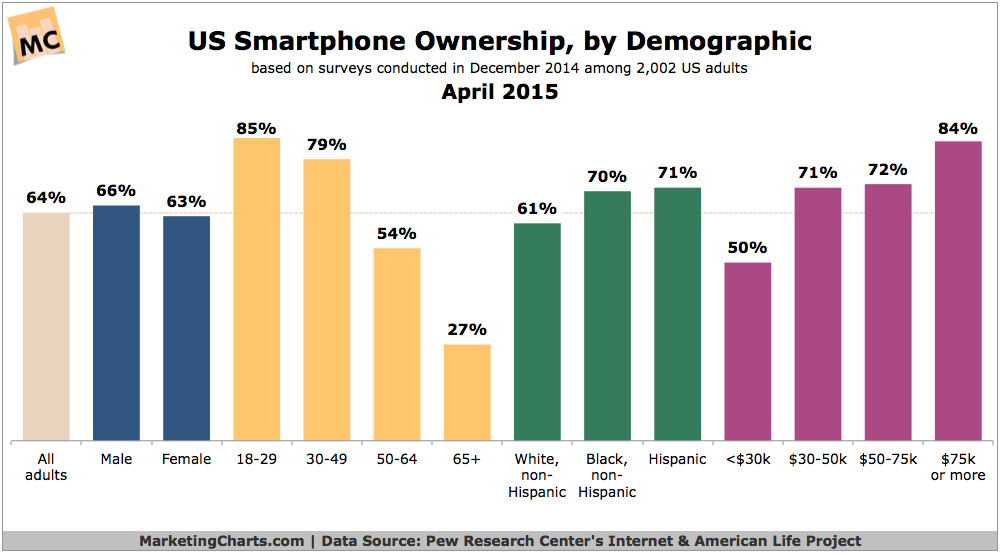
\includegraphics[scale=0.3]{img/demographic-smartphone.png}
\end{figure}
Dal grafico si envince che la ormai l'utilizzo degli smartphone è
estremamente diffuso in quasi tutte le categorie demografiche.
I meno soggetti all'utilizzo di smartphone sono gli individui con un età
che supera i 65 anni.

\begin{minipage}{0.45\textwidth}
\item
Crescita di interesse per la cucina.\\
Recenti articoli parlano di come
ci sia sempre più interesse verso l'arte culinaria. 
Si può riscontrare anche dal gran numero di programmi televisi in voga
negli anni. Inoltre si possono incontrare sempre più blog e canali
youtube nel web di appassionati di cucina che condividono le loro
ricette ed esperimenti.
La condivisione è una proprietà intrinseca della passione culinaria: le
nostre nonne hanno sempre conservato il libro delle ricette personali da
ampliare con le collezioni di ricette passate da amiche e parenti.
Indubbiamente questo fenomeno è esploso con il web e c'è sicuramente
spazio di mercato per applicazioni che permettono di coltivare la
passione culinaria.
\end{minipage}
\begin{minipage}{0.45\textwidth}
\begin{figure} [H]
	\centering
	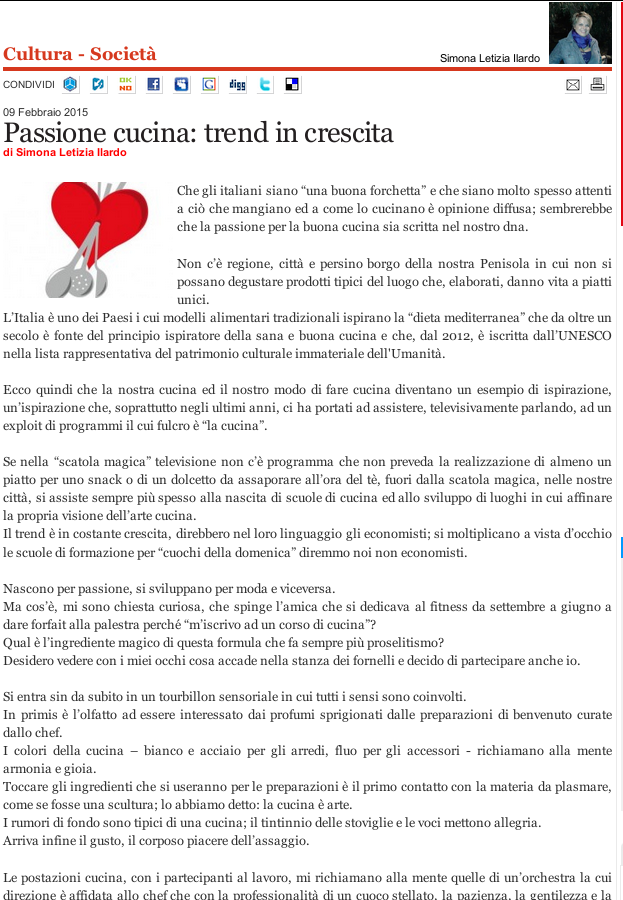
\includegraphics[scale=0.3]{img/articolo-cucina.png}
\end{figure}
\end{minipage}

La figura \ref{fig:demographic-coockapp} riassume uno studio statistico
condotto in Gran Bretagna nel 2013 che mostra la diffusione
dell'utilizzo di applicazioni per cucinare caratterizzata per età e
sesso. In particolare si può notare che c'è un maggiore utilizzo da
parte delle donne e per le persone sotto i 50 anni anche se la
distribuzione di utilizzo è piuttosto omogenea.

\begin{figure}[H]
	\centering
	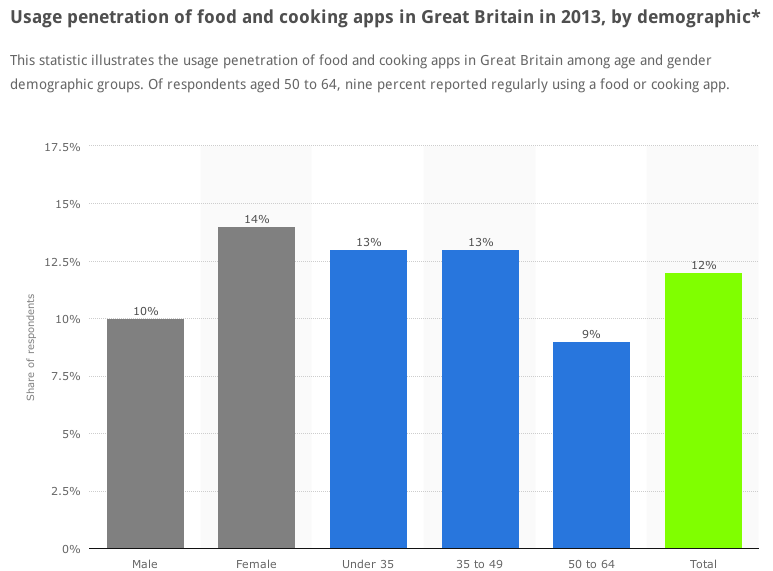
\includegraphics[scale=0.3]{img/demographic-cookapp.png}
	\caption{Diffusione demografica delle applicazioni culinarie in Gran Bretagna nel
2013}	
	\label{fig:demographic-cookapp}
\end{figure}

Inoltre come si evince dalla figura \ref{fig:cooking-country}, ci sono
nazioni in cui la passione per la cucina è importante a differenza di
altre. In particolare l'Italia risulta essere prima in classifica per
passione culinaria.
Questo suggerisce la possibilità di progettare un'applicazione culinaria
specifica per la cucina italiana, la quale da se offre sicuramente un mercato
interessante, senza però escludere la possibilità di
coltivare la passione per la cucina internazionale. 
Un approccio meno specifico e più internazionale rischierebbe di
confondere l'utente medio italiano più legato ai ricettari classici
della cucina italiana. 

\begin{figure}[H]
	\centering
	
\includegraphics[scale=0.7]{img/cooking-country.jpg}
	\caption{Nazioni a confronto riguardo la passione culinaria}	
	\label{fig:cooking-country}
\end{figure}

\end{itemize}

Da quanto visto emerge un target ideale d'utilizzo che si differenzia per ogni
caratteristica demografica:
\begin{itemize}
\item \textbf{Età}. La fascia d'età di maggior interesse è dai 13-65
anni. Non esclude gli over 65 se con una particolare predisposizione
alla tecnologia.
\item \textbf{Sesso}. Qualsiasi: anche se le donne hanno mostrato avere più
interesse nella cucina rispetto agli uomini, il divario è minimo e rende
così l'applicazione indipendente dal sesso.
\item \textbf{Reddito}. Qualsiasi:
in genere le ricette presenti nelle applicazioni culinarie hanno diverse
fasce di prezzo rendendo quest'ultime indipendenti dal reddito dell'utente.
\item \textbf{Nazionalità}. Prevalentemente italiana. Non esclude gli
appassionati per la cucina italiana di diversa nazionalità.
\item \textbf{Istruzione}. È sufficiente possedere una cultura di base sulla terminologia
culinaria e sulla conoscenza delle materie prime più comuni. Si prevede
ovviamente che l'utente sia alfabetizzato e che comprenda le lingue
dell'applicazione. 

\end{itemize}

\subsubsection{Segmentazione Psicografica}
Al fine di identificare al meglio le tipologie di
utenti interessati all'applicazione proposta, abbiamo segmentato
ulteriormente l'utenza, in questo caso individuando le loro caratteristiche
psichiche.

\begin{itemize}
\item \textbf{Intraprendente}
L'applicazione potrebbe incuriosire quegli utenti che, nonostante il
basso livello di competenza tecnologica, non hanno paura di sperimentare
nuovi aspetti della vita quotidiana. In genere si parla degli
intraprendenti che, determintati ad ottenere una certa soluzione, non si
frenano davanti alle difficoltà.
\item \textbf{Insicuro}
Spesso si vedono amanti della cucina non molto abili dietro i fornelli,
a volte per lacune tecniche oppure perchè mancano di sicurezza.
Quest'ultimi si riconoscono dalla minuziosità nel rispettare le dosi di
una ricetta e dalla paura di azzardare qualche punta di
personalizzazione.
Un'applicazione in grado di fornire delle ricette da cucina ad un alto
livello di dettaglio e suggerrimenti su come poter personalizzarle,
sarebbe sicuramente attraente per gli utenti insicuri.
\item \textbf{Ansioso}
Solitamente le persone ansiose hanno difficoltà nell'organizzazione di
cene domestiche. Ad esempio può accadere che tali persone si portino troppo avanti
con le preparazioni per evitare di non far attendere i loro ospiti, ma
potrebbero servire piatti freddi o eseguiti male se presi dal panico.
Un'applicazione che oltre a fornire delle ricette riesca anche a
pianificare dettagliatamente l'organizzazione di una cena potrebbe essere
interessante per gli utenti ansiosi.
\item \textbf{Curioso}
Spesso i buon gustai si chiedono come vengano preparati i loro piatti
preferiti. Questa è la categoria dei curiosi che potrebbero avvalersi di
un app da cucina per investigare sulle ricette che gli stuzziccano
l'interesse.
\item \textbf{Salutista}
Si vedono sempre più di frequente persone interessate a seguire un
alimetazione sana. In genere i salutisti sono coloro che fanno jogging
al parco, vanno in palestra tutti i giorni e stanno attenti alla linea.
La categoria però comprende anche coloro che, facendo poca attività
fisica, cercano di migliorare la loro qualità di vita con una dieta intenta 
a limitare la quantità di grassi assunti.
Per i salutisti un applicazione che li guidi alla ricerca di ricette e
piatti compatibili con la loro alimentazione scelta potrebbe essere
molto interessante.

\end{itemize}


\subsection{User Research}
Con l'obiettivo di avere un'idea più chiara riguardo le carittistiche
principali di usabilità dell'applicazione proposta, verrà analizzata di
seguito l'esito dell'attività di user research.

\subsubsection{Market Research}
Abbiamo preparato e pubblicato un sondaggio da far compilare ad un
insieme eterogeneo di persone. Abbiamo creato il questionario tramite
l'applicazione Google Form ed è stato compilato da 148
soggetti diversi.\\

Nello specifico riportiamo le domande e le relative risposte.
\begin{itemize}
	\item\textbf{Anagrafica}
		\begin{figure} [H]	
			\centering
			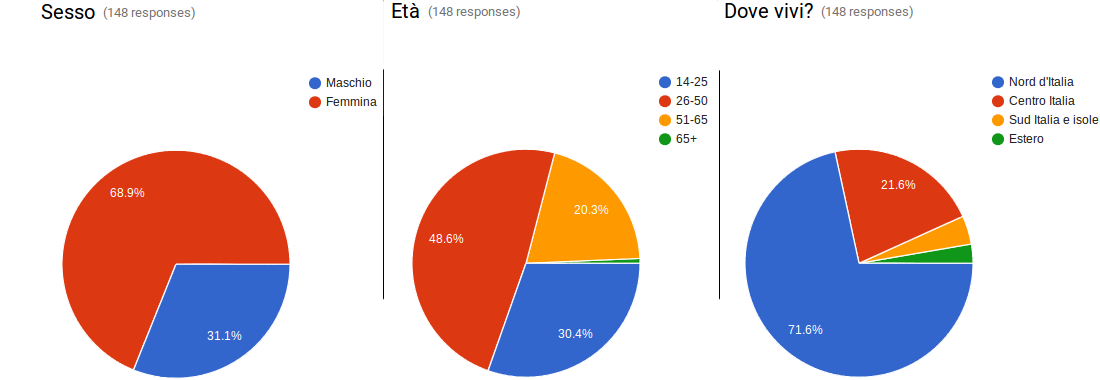
\includegraphics[width=\textwidth]{img/survey-123.png}
		\end{figure}
	\item\textbf{Competenze in Cucina}
		\begin{figure} [H]	
			\centering
			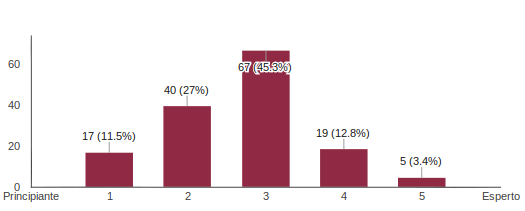
\includegraphics[scale=0.65]{img/survey-4.png}
		\end{figure}
	\item\textbf{Utilizzo Dispositivi in Generale}
		\begin{figure} [H]	
			\centering
			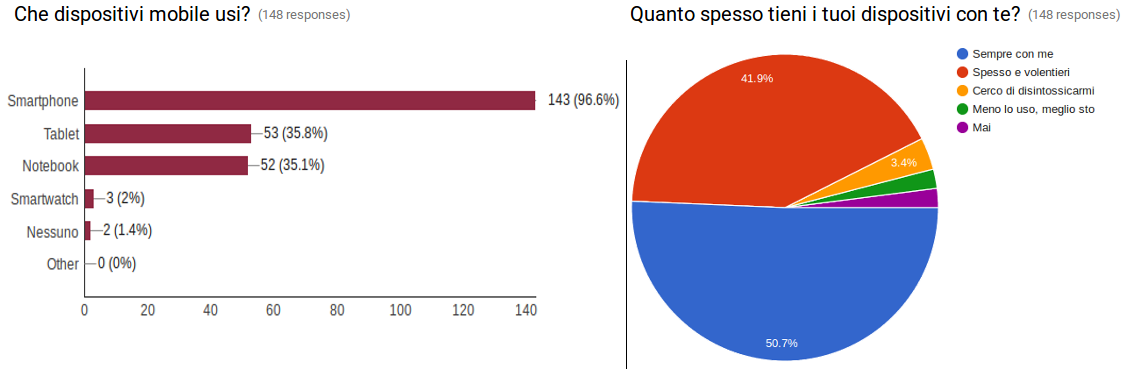
\includegraphics[scale=0.45]{img/survey-56.png}
		\end{figure}
	\item\textbf{Utilizzo Dispositivi in Cucina}
		\begin{figure} [H]
			\centering
			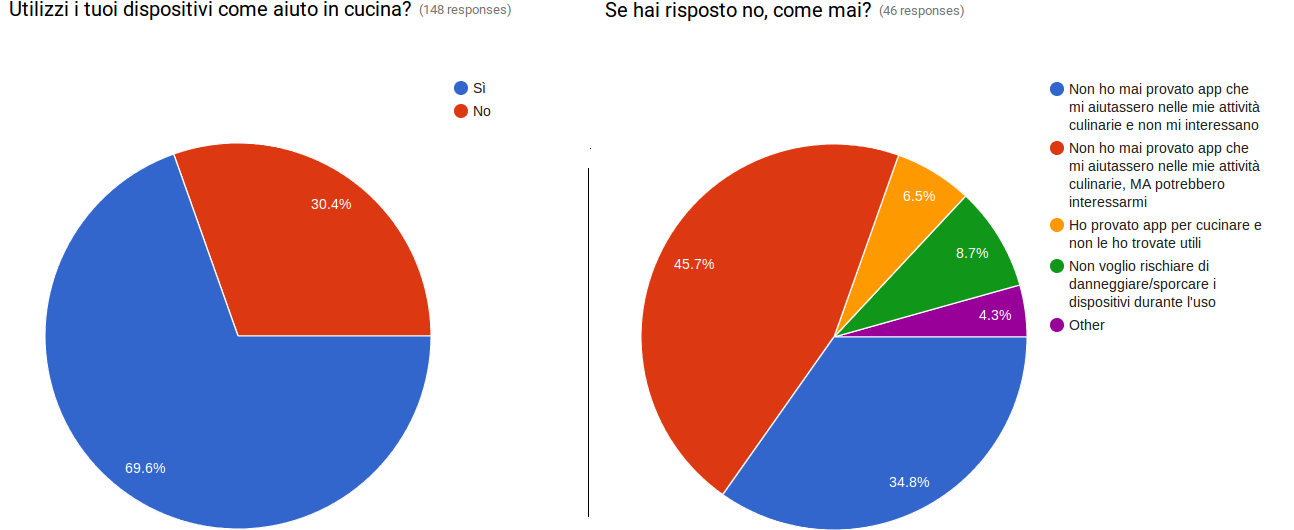
\includegraphics[scale=0.40]{img/survey-78.png}
		\end{figure}
		
		\begin{figure} [H]
			\centering
			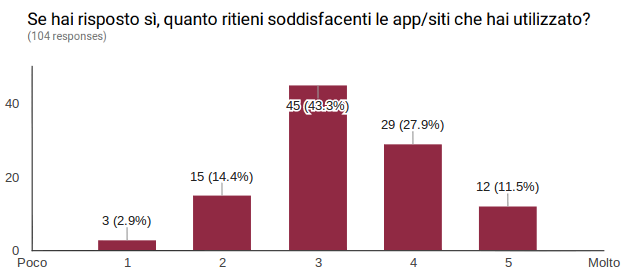
\includegraphics[scale=0.55]{img/survey-9.png}
		\end{figure}
	\item\textbf{Le funzioni che trovano o troverebbero più utili gli
utenti in un app per cucinare}\\
		Le risposte possibili erano le seguenti:
		\begin{enumerate}
			\item Un buon catalogo di ricette
			\item Le videoricette
			\item I consigli della cummunity
			\item La possibilità di creare liste della spesa di ricette
			\item La possibilità di organizzare un pasto completo
tramite l'abbinamento di ricette
			\item La possibilità di controllare i procedimenti tramite
comandi vocali
			\item Altro (risposta libera)
		\end{enumerate}
		\begin{figure} [H]
			\centering
			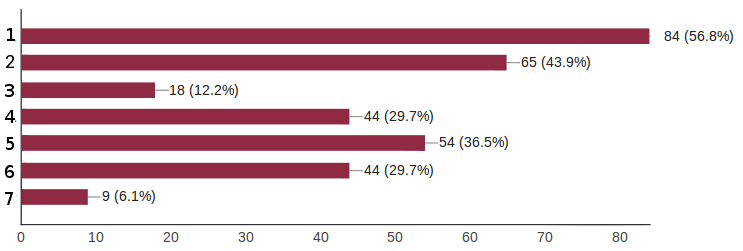
\includegraphics[scale=0.55]{img/survey-10.png}
		\end{figure}
	Le proposte più interessanti tra quelle a risposta libera sono
state: "La possibilità di ricavare ricette dagli ingredienti
disponibili" e "La possibilità di scegliere le ricette in base a
intolleranze" la quale è stata proposta da più utenti anche se in forme
leggermente diverse.
	\item \textbf{Lista della spesa}
		\begin{figure} [H]
			\centering
			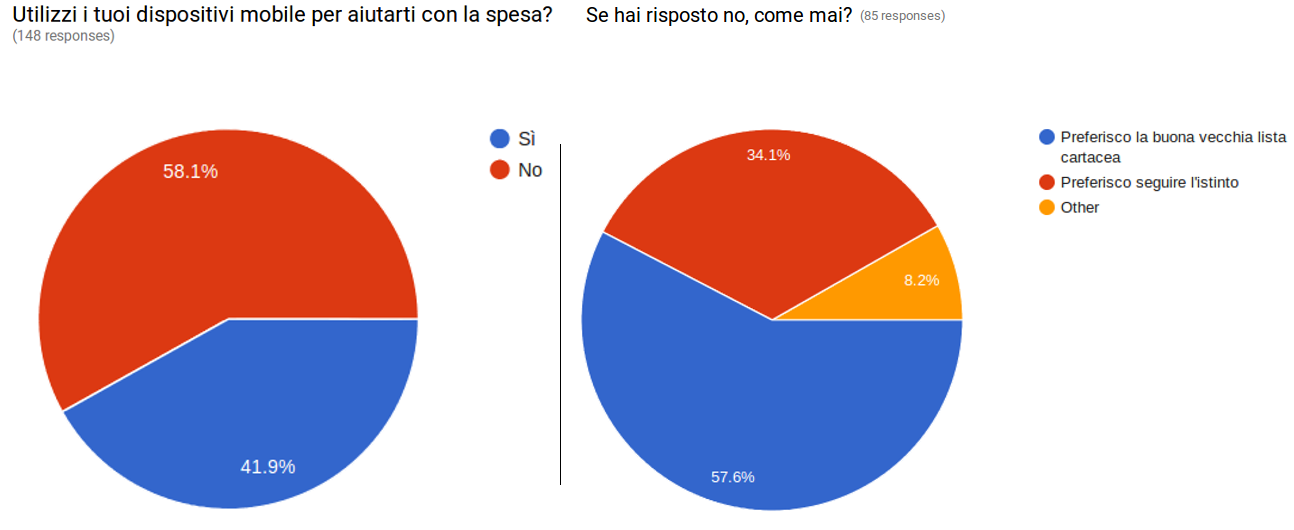
\includegraphics[scale=0.40]{img/survey-1112.png}
		\end{figure}
	Nelle spiegazioni alle risposte negative, la maggior parte delle
persone che ha risposto "Altro" ha indicato che non in genere non
utilizza affatto liste delle spesa.
\end{itemize}

Sommariamente il sondaggio ha coinvolto un gruppo di persone di sesso
femminile predominante, età principalmente dai 14-50 anni e concentrati
nel nord e centro Italia.\\
Il pool di esaminati ha definito mediamente di avere competenze culinarie
medio-basse e come aspettato di essere molto dipendete dai dispositivi
mobili più comuni in commercio. \\

Inoltre, circa il 70\% di loro ha dichiarato di
utilizzare tali dispositivi come aiuto in cucina trovandole mediamente
soddisfacenti. Il restante
30\% invece non utilizza dispositivi mobili in cucina, ma 
quasi la metà di loro sarebbe interessata ad utilizzarli non avendo però
mai provato applicazioni per cucinare.
In aggiunta, gli esaminati trovano estremamente interessante
applicazioni che offrono un buon catalogo di ricette e videoricette.
Scaturiscono anche discreto interesse funzionalità per creare liste
della spesa, organizzare menu completi abbinando più ricette e il
controllo dell'applicazione tramite comandi vocali. Invece viene presa
poco in considerazione il supporto da parte della community.
Infine i soggetti esaminiti si dividono quasi per le metà tra chi
utilizza dispositivi mobili per fare la spesa e chi invece no, con una
piccola prevalenza per questi ultimi.\\

Da questa ricerca di mercato evince che c'è sicuramente domanda per
questo tipo di applicazioni e margine di miglioramento rispetto ai prodotti
già esistenti considerando i livelli di soddisfazione delle persone
esaminate.
\subsubsection{Contextual Inquiry}
Vedremo qui di seguito due osservazioni effettuate sul campo d'azione
di alcuni potenziali utenti, al fine di individuare dettagli importanti
dipendenti dal contesto d'utilizzo dell'applicazione.

\begin{enumerate}
\item Dario, Paolo e Giacomo sono tre coinquilini universitari, svegli ma non molto
abili in cucina. Nonostante la loro poca esperienza, occasionalmente
decidono di cimentarsi nella preparazione di qualche ricetta trovata
online, sia per rompere la monotonia della classica pasta con il tonno,
sia per avere una valida distrazione dallo studio.
Sono stati osservati nel tentativo di preparazione di un dolce.
Inizialmente i tre hanno deciso di far pranzo con delle
tagliatelle all'arancia, una delle prime ricette trovate online che ha risvegliato il
loro appetito. Seguendo nel dettaglio la ricetta hanno portato a termine
con successo la preparazione delle tagliatelle gustandosi un buon
pranzo insolito. 
Quella mattina però al supermercato non vendevano
arance sfuse e hanno dovuto per forza acquistare la confezione grande.
Inoltre la ricetta delle tagliatelle prevedeva l'utilizzo di soltanto i
tuorli delle uova così che i tre studenti si sono ritrovati con un
eccesso di arance e albumi dopo il pranzo.

Mossi dalla loro grande voracità e dall'alternativa di un triste pomeriggio sui libroni di
matematica hanno deciso di cercare online un dolce all'arancia.
Hanno deciso quindi di tentare la preparazione di una mousse
all'arancia. La ricetta richiedeva però la colla di pesce, ingredienti non di uso
quotidiano per tre studenti universitari abituati ad ordinare persino il
dolce a domicilio. Troppo sicuri delle loro intuizioni hanno però
provato lo stesso a preparare la mousse utilizzando gli albumi montati a
neve in sostituzione alla colla di pesce. 

Al termine della preparazione hanno preso atto che la consistenza non era adatta ad una mousse. 
Hanno deciso quindi di aggiungere del cacao amaro in
polvere al composto senza alcuna ragione reale ma spinti piuttosto dalla curiosità e divertiti
dall'improvvisazione. Mescolando però ulteriormente l'impasto hanno smontato
gli albumi. A quel punto affranti dall'eventualità di non poter gustare
alcun dolce hanno deciso di ripiegare disperati su una torta
``facciopresto'' consigliata telefonicamente da una loro amica. Hanno
quindi infine aggiunto farina e burro all'impasto e infornato il tutto
ottenendo in ultimo un risultato qualitativamente molto scarso.
Ovviamente Dario, Paolo e Giacomo, ormai stanchi e affamati, hanno comunque consumato interamente la
torta non desiderata, sognando ad ogni morso una deliziosa mousse all'arancia.

\item Antonietta è un'impiegata di 48 anni del sud Italia. È una signora che
nella sua vita ha viaggiato poco ed è molto legata alle tradizioni della
sua terra d'origine. Da quando i suoi figli hanno lasciato casa per
studio e lavoro, Antonietta ha iniziato ad interessarsi di più alla
ricerca culinaria e alla sperimentazione di piatti che si distaccassero
dalle sue tradizioni.\\

La signora Antonietta è stata osservata durante la preparazione della polenta taragna, un
piatto tipico valtellinese la cui ricetta è stata da lei trascritta dopo
averne visto la preparazione in un programma culinario televisivo.

Antonietta inizia la preparazione del piatto seguendo minuziosamente le
dosi della ricetta e pesando nel dettaglio ogni ingrediente. Casualmente
quel giorno era in casa anche sua sorella Roberta che ha un amica,
Elisa, originaria del nord Italia trasferitasi in puglia dopo il matrimonio.
Roberta ha visto una volta preparare la polenta taragna da Elisa e
ricorda che per la preparazione della polenta taragna occorrono circa 5
bicchieri di farina per una forma piccola di formaggio. La signora
Antonietta non si fida molto della memoria e della sicurezza di sua sorella
e vuole procedere per la strada della ricetta. Le due discutono per
diverso tempo sul corrispettivo in grammi di 5 bicchieri di farina e su
sul tipo di bicchieri da prendere in considerazione per tale
conversione. Fanno anche diverse prove con vari bicchieri in quanto la
signora Antonietta non aveva lo stesso identico modello di bicchieri della
signora Elisa. Infine Antonietta perde la pazienza e continua per la sua
strada utilizzando il dosaggio in grammi indicato nella ricetta. La
preparazione del piatto viene terminata con successo e con un'ottima
polenta taragna, anche se le due sorelle non la gustatano al meglio avendo
gli animi ancora alterati dalla precedente discussione.
\end{enumerate}

Analizzando le due osservazioni emergono dei dettagli di usibilità da
tenere in considerazione.

Nel caso dei tre studenti una buona
applicazione avrebbe potuto suggerire un ingrediente opportuno in
sostituzione alla colla di pesce. Inoltre con la possibilità di chiedere
aiuto alla community, l'app avrebbe dato la possibilità ai tre ragazzi di capire in
anticipo che gli albumi delle uova montati a neve non sono opportuni per
una mousse sotto suggerimento di qualche altro utente.

Per quanto riguarda la signora Antonietta, se avesse usato un'applicazione 
da cucina con una funzionalità di conversione da grammi a
bicchieri, avrebbe evitato di discutere con la sorella. In
alternativa avrebbe anche potuto chiedere conferma agli
utenti valtellinesi della community della correttezza delle dosi scritte
nella ricetta.

\subsubsection{Task Analisys}
Di seguito la lista dei task principali che abbiamo individuato per un'applicazione da
cucina:
\begin{enumerate}
\label{tasks}
\item Ricerca di una ricetta per nome.
\item Ricerca di una ricetta per ingredienti.
\item Filtro di una ricetta per categoria.
\item Filtro di una ricetta in base alle intolleranze/allergie.
\item Suggerimenti sulle ricette di stagione.
\item Salvare una ricetta nei preferiti.
\item Rimuovere una ricetta dai preferiti.
\item Distinguere le varie fasi di una preparazione della ricetta.
\item Visualizzare le foto inerenti alla preparazione di
una ricetta.
\item Avanzare con le fasi di preparazione mediante messaggi vocali.
\item Text-to-Speech delle fasi di preparazione di una ricetta.
\item Individuare gli ingredienti necessari alla preparazione di una
ricetta.
\item Individuare la difficoltà di preparazione di una ricetta.
\item Inserire una nuova ricetta nel catalogo dell'applicazione.
\item Condividere una ricetta sui social network.
\item Commentare una ricetta in un apposito topic online.
\item Accedere alla lista della spesa.
\item Inserire gli ingredienti nella lista della spesa.
\item Rimuovere gli ingredienti dalla lista della spesa.
\item Modificare la grandezza del font di una ricetta.
\item Creare un menù completo selezionando una lista di ricette.
\item Selezionare la lingua dell'applicazione.
\end{enumerate}

Vedremo in seguito gli approcci delle applicazioni già esistenti verso
questi task e le funzionalità da progettare nella nostra applicazione
affinché tali task possano essere eseguiti al meglio.

\documentclass[12pt,a4paper,openright,twoside]{article}

\usepackage[italian]{babel}

\usepackage[utf8x]{inputenc}
\usepackage{caption}
\usepackage{geometry}
\usepackage{float}
\usepackage{wrapfig}
\usepackage{graphicx}
\usepackage{caption}
\usepackage{subcaption}
\usepackage{listings}
\usepackage{color}

\usepackage{mwe}
\usepackage{graphbox} %loads graphicx package


\usepackage{fancyhdr}


\usepackage{indentfirst}

\usepackage{graphicx}

\usepackage{newlfont}

\usepackage{amssymb}
\usepackage{amsmath}
\usepackage{latexsym}
\usepackage{amsthm}

\usepackage{mathtools}
\usepackage{pdfpages}

\usepackage{subfig}

\begin{document}

\section{Valutazione di sistemi esistenti}

In questa fase si sono analizzate applicazioni concorrenti già inseriti nei market più famosi di dispositivi mobili, per evidenziare problemi di usabilità (metriche quantitative e qualitative di usabilità utili come input per la fase di design e per un confronto successivo).\\
Individuata la categoria più adatta (\textit{Stile di vita} su \textit{Google Play Store} / \textit{Ristoranti e bar} su \textit{Microsoft Store}), abbiamo individuato due app strutturalmente
diverse, ma che a prima analisi sono dei buoni modelli di partenza al fine di progettare la nostra applicazione.\\
Abbiamo analizzato:
\begin{itemize}
\item \textbf{”Giallo Zafferano”}\\
Sviluppatore: Banzai Media\\
Installazioni: 1.000.000-5.000.000 su Google Play\\
Piattaforme compatibili: Android, iOS, Windows Phone/Store\\
Punteggio: 4,2/5 su 26.621 recensioni\\
Versione analizzata: app tablet Windows Store\\
Lingua: Italiano\\
\item \textbf{”Allthecooks”}\\
Sviluppatore: Allthecooks, LLC.\\
Installazioni: 10.000.000-50.000.000 su Google Play\\
Piattaforme compatibili: Android, iOS, Windows Phone/Store, Smartwatch\\
Punteggio: 4,3/5 su 46.678 recensioni\\
Versione analizzata: app tablet Windows Store\\
Lingua: Inglese\\
\end{itemize} 

\subsection{Expert Usability Review}
Procediamo ora con l'expert usability review, ovvero l'analisi dell'usabilità di un software o piattaforma web da parte di un esperto di usabilità. A tal proposito ci avvarremo del consulto di Alessandro D'Andrea, Business Analyst di Yoox.com, al fine di verificare pregi e difetti dell'usabilità riscontrati nelle due applicazioni.\\
L'analisi si divide in diverse fasi:
\begin{itemize}
\item Definizione delle linee guida adatte e prima dell'esplorazione
\item Analisi dell'architettura
\item Analisi diretta: sistema VS linee guida
\item Analisi inversa: linee guida VS sistema
\item Rilevazione di un numero ragionevole di errori
\item Identificazione dei task del sistema
\item Identificazione del target di utenza
\end{itemize}

\subsection{Le linee guida utilizzate}
Internamente al team abbiamo deciso di utilizzare le 10 euristiche di Nielsen e Molich come linee guida, approfondite e adattate al nostro contesto, al fine di valutare preventivamente l’usabilità del sistema rispetto ai task che vogliamo raggiungere.\\
Abbiamo quindi valutato i seguenti parametri:
\begin{enumerate}

\item Visibilità dello stato del sistema\\
Il sistema dovrebbe sempre tenere informato l’utente su quel che succede,
attraverso feedback appropriato fornito in tempi ragionevoli; ogni sezione e ogni fase della preparazione della ricetta devono essere chiari e visibili in ogni momento.

\item Match tra il sistema e il mondo reale\\
Il sistema dovrebbe parlare il linguaggio dell’utente, con parole, frasi e
concetti familiari all’utente piuttosto che termini sistemistici. Deve seguire
convenzioni del mondo reale, e far comparire le informazioni in un ordine
naturale e logico. Si ricorda che l'uso è destinato a utenti di esperienza culinaria diversa: il sistema si deve adattare di conseguenza ad un lessico più semplice per i principianti o più tecnico per i maestri dei fornelli. \\

\item User control e libertà\\
Poichè l’utente spesso sceglie funzioni di sistema per errore, ha bisogno
di ”uscite di sicurezza” ben visibili per abbandonare lo stato non voluto
senza dover passare per un dialogo complesso. Supportare undo e redo soprattutto nelle fasi di preparazione di una ricetta.\\

\item Coerenza e standard\\
Gli utenti non dovrebbero chiedersi se parole, situazioni e azioni diverse
hanno significati simili o producono azioni simili. Seguire le convenzioni
della piattaforma.\\

\item Prevenzione degli errori\\
Ancora meglio di un buon messaggio d’errore è una cura progettuale adeguata a prevenire che accadano gli errori. Eliminare le condizioni che portano ad errori o controllarne l’occorrenza e presentare all’utente una richiesta di conferma prima che si impegnino nell’azione corrispondente.\\

\item Recognition piuttosto che recall\\
Minimizzare il carico di memoria dell’utente rendendo visibile oggetti,
azioni ed opzioni dell’interfaccia. Gli utenti non dovrebbero essere costretti a ricordare informazioni da una parte all’altra del dialogo. Le istruzioni per l’uso del sistema dovrebbero essere visibili o facilmente recuperabili quando necessario. Il sistema deve quindi essere dotato di una sezione help facilmente consultabile.\\

\item Flessibilità ed efficienza d’uso\\
Acceleratori nascosti all’utente novizio possono velocizzare l’interazione
degli utenti esperti in modo da favorire sia gli utenti senza e con esperienza.
Permettere agli utenti di personalizzare le azioni frequenti come la possibilità di avere una sezione di ricette preferite.\\

\item Estetica e design minimalista\\
I dialoghi non debbono contenere informazioni irrilevanti o raramente utilizzate. L'interfaccia non deve essere troppo ricca di contenuti e ogni sezione deve essere facilmente raggiungibile.\\

\item Aiutare gli utenti a riconoscere, diagnosticare, e recuperare gli errori\\
I messaggi d’errore debbono essere espressi in linguaggio semplice (senza codici e tecnicismi), debbono indicare precisamente il problema e suggerire costruttivamente una soluzione.\\

\item Help e documentazione\\
E' meglio quando il sistema può essere usato senza documentazione. Laddove sia necessario o opportuno fornirla, le informazioni debbono essere facili da cercare, focalizzate sui task dell'utente, elencare passi concreti da svolgere e non essere troppo lunghe da leggere. 
\end{enumerate}

\subsection{Analisi delle applicazioni}
Per entrambe le applicazioni abbiamo cercato di analizzare l'usabilità e l’esperienza
utente che ne deriva mentre si passa da una schermata all’altra. Si è inoltre valutato se le
applicazioni proposte implementavano funzionalità quali l’interazione sociale tra gli utenti, la
lingua e la comprensibilità dei testi.\\
A livello di contenuti abbiamo verificato la qualità della proposta delle ricette come l’esperienza nel trovarle nel sistema ed eventualmente comporle per l'organizzazione di un pasto completo.\\
Infine la verifica dell'interazione sociale: ci si è chiesti se i competitors avessero
possibilità di interazione tramite social network, valutazione delle ricette, commenti alle stesse e
la possibilità di richiedere alla comunità suggerimenti in merito alle preparazioni e consigli in
genere.
\subsubsection{GialloZafferano}

GialloZafferano è senza dubbio uno dei punti di riferimento del web italiano per quanto riguarda le passioni culinarie: con oltre 5,6 milioni di app scaricate, oggi raccoglie più di 3000 ricette e suggerimenti per ogni tipologia di palato.\\
L'app per Windows Store è sotto certi versi quella più acerba tra i vari store mobile, caso di studio ideale per la nostra analisi.\\

\begin{figure}[h]
  \makebox[\textwidth][c]{\includegraphics[width=1\textwidth]{./Giallozafferano/Home.png}}%
  \caption{Schermata principale}
  \label{fig:key}
\end{figure}

La schermata principale occupa circa la metà dello spazio totale dello schermo e propone il menù della settimana insieme alle varie categorie di ricette, i preferiti e la lista della spesa (se compilata). Inoltre una discreta barra di ricerca permette di cercare una ricetta dal nome.

\begin{figure}[h]
  \makebox[\textwidth][c]{\includegraphics[width=1\textwidth]{./Giallozafferano/menu.png}}%
  \caption{Il menù superiore}
  \label{fig:key}
\end{figure}

Lo scroll dal margine alto verso il centro, permette di accedere al menù dell'applicazione, altrimenti nascosto.\\
Le scelte disponibili sono: la visualizzazione della home, il menù della settimana, la schermata delle categorie, i preferiti e la lista della spesa.\\

\begin{center}
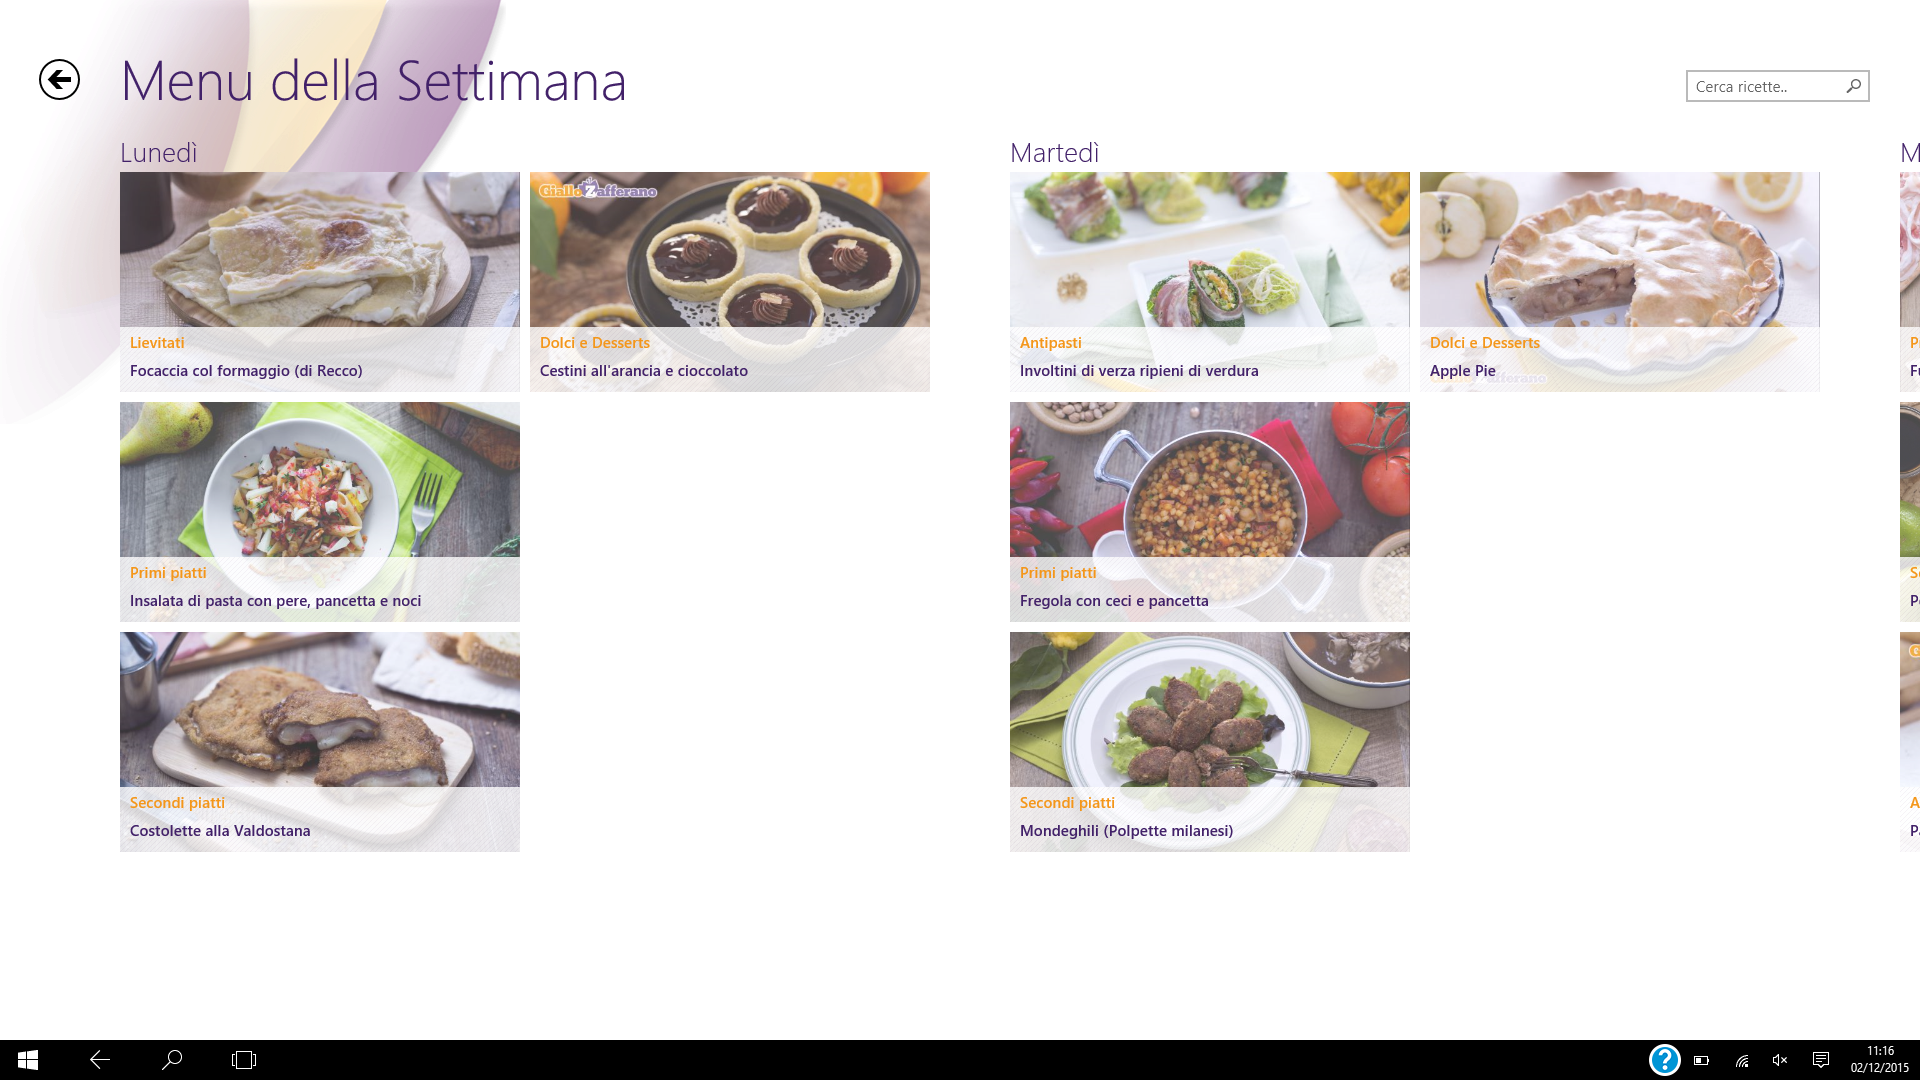
\includegraphics[scale=0.25] {./Giallozafferano/menu_settimana.png}  
\captionof{figure}{Schermata menù della settimana (scroll orizzontale)\\}
\end{center}

\begin{center}
\includegraphics[scale=0.3] {./Giallozafferano/categorie.png}  
\captionof{figure}{Schermata categorie\\}
\end{center}

\begin{center}
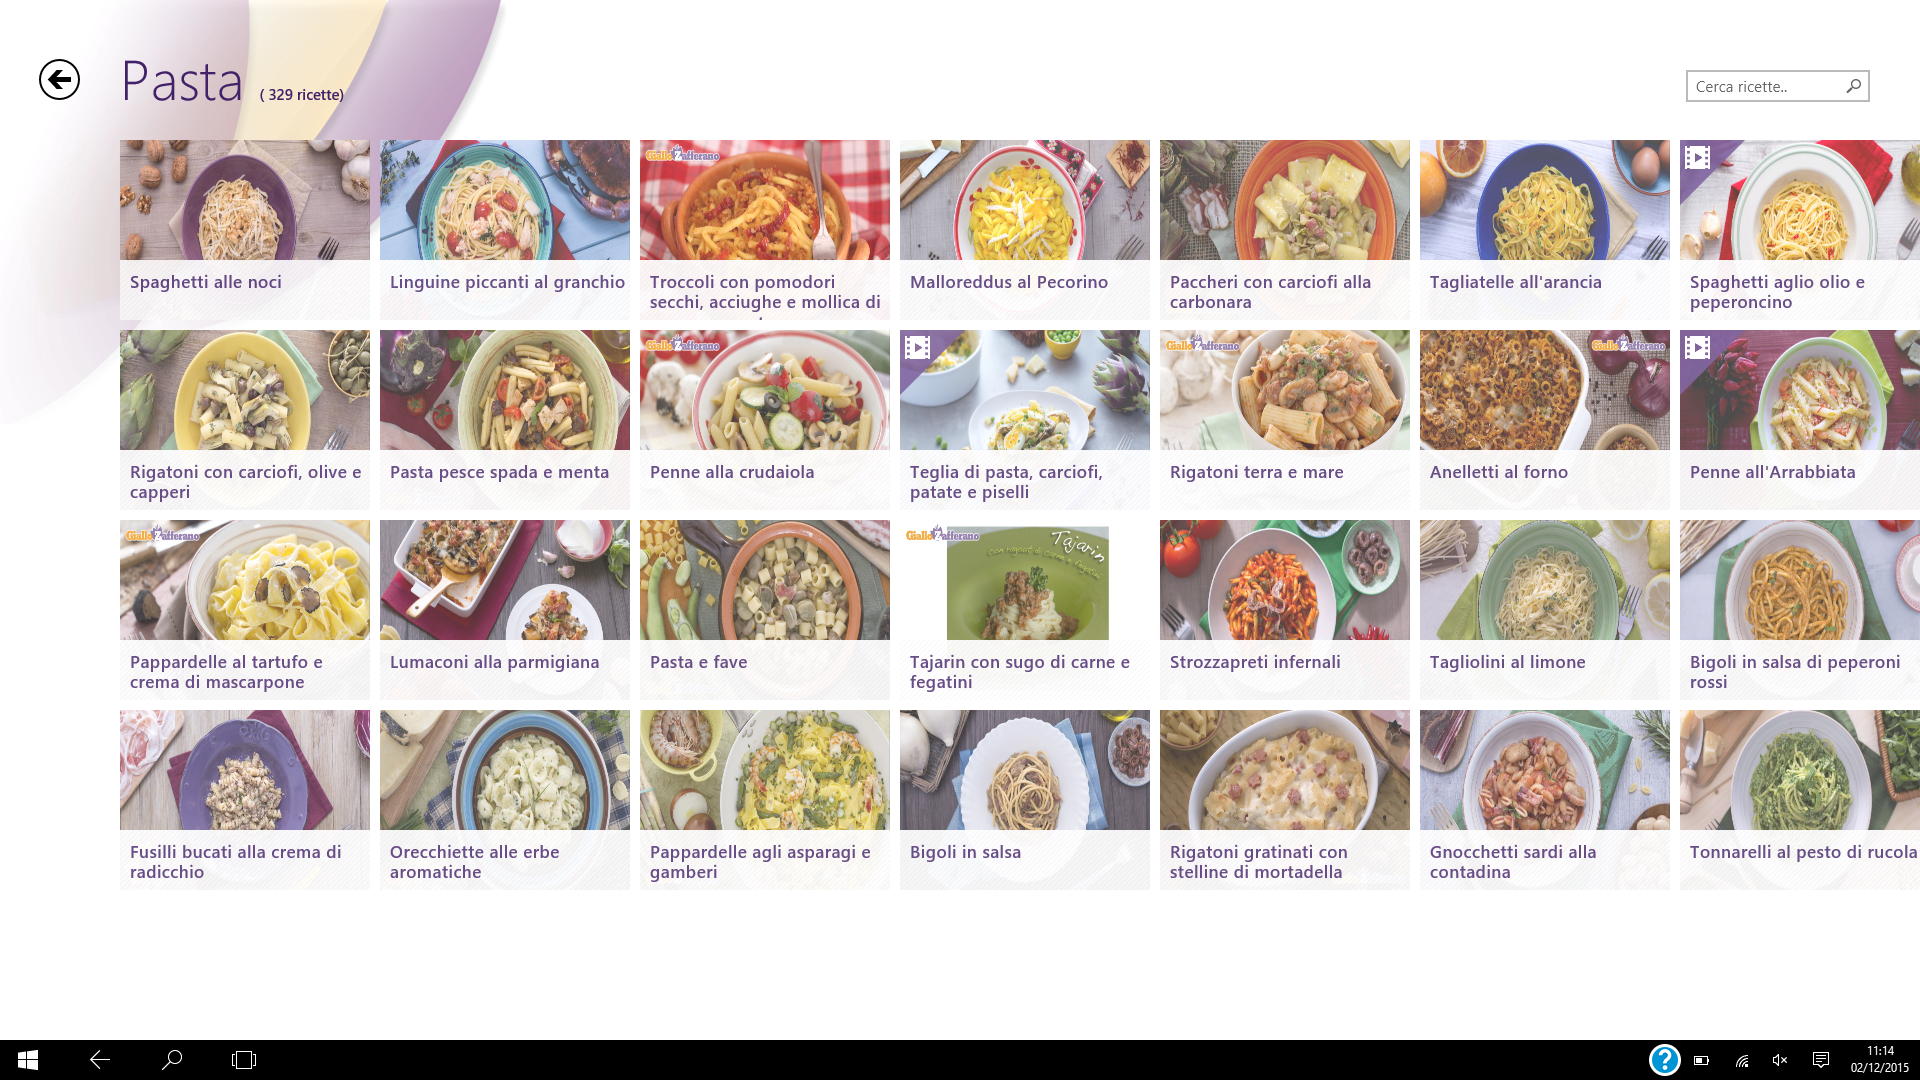
\includegraphics[scale=0.3] {./Giallozafferano/pasta.png}  
\captionof{figure}{Schermata primi piatti : pasta (scroll orizzontale)\\}
\end{center}


L'interfaccia destinata alla presentazione della ricetta risulta ricca di informazioni, con alcuni difetti: nella parte sinistra si propone la videoricetta (se disponibile), insieme alle informazioni base come difficoltà, tempo di cottura e preparazione, ingredienti; scrollando a destra è visionabile la procedure la procedura di preparazione con immagini, conservazione e curiosità.

\begin{center}
\includegraphics[scale=0.275] {./Giallozafferano/ricetta.png}  
\captionof{figure}{Un esempio...\\}
\end{center}

\begin{center}
\includegraphics[scale=0.275] {./Giallozafferano/ricetta_2.png}  
\captionof{figure}{...di ricetta\\}
\end{center}

Anche qui è possibile visualizzare il menù, scrollando dal borso superiore al centro.

\begin{center}
\includegraphics[scale=0.275] {./Giallozafferano/ricetta_menu.png}  
\captionof{figure}{...di ricetta\\}
\end{center}

Il menù superiore non presenta differenze da quello analizzato precedentemente; quello inferiore ha tre funzioni: "\textit{Pin to Start}" per aggiungere la ricetta ai preferiti del sistema operativo, \textit{"Aggiungi ai preferiti"} dell'applicazione e \textit{"Aggiungi alla lista della spesa"}.\\\\
\newpage
Ogni utente ha la possibilità di inserire note personali (private) cliccando sulla matita.

\begin{center}
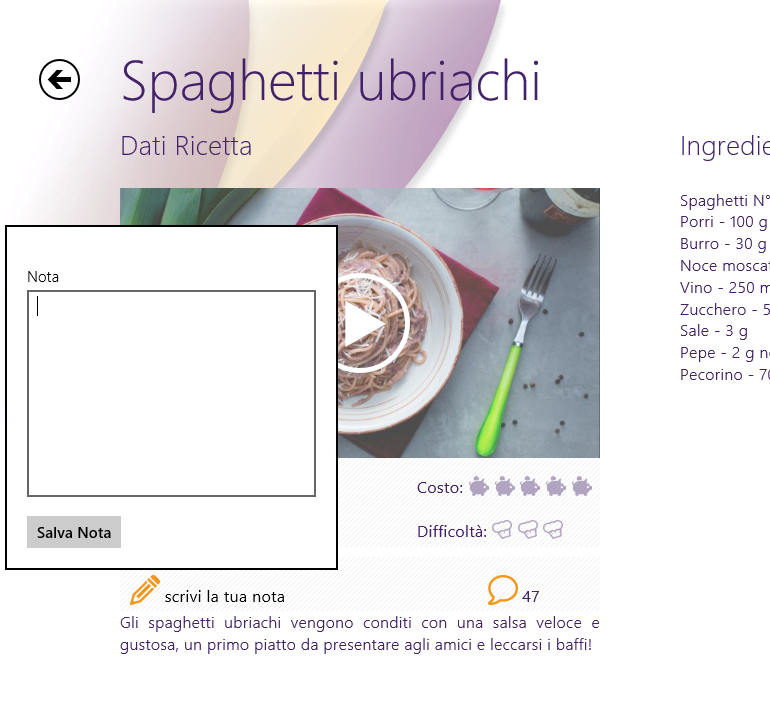
\includegraphics[scale=0.4] {./Giallozafferano/ricetta_nota.png}  
\captionof{figure}{Inserimento di una nota\\}
\end{center}

E' inoltre possibile partecipare ai commenti online per confrontarsi con altri utenti e/o offrire/cercare assistenza.

\begin{center}
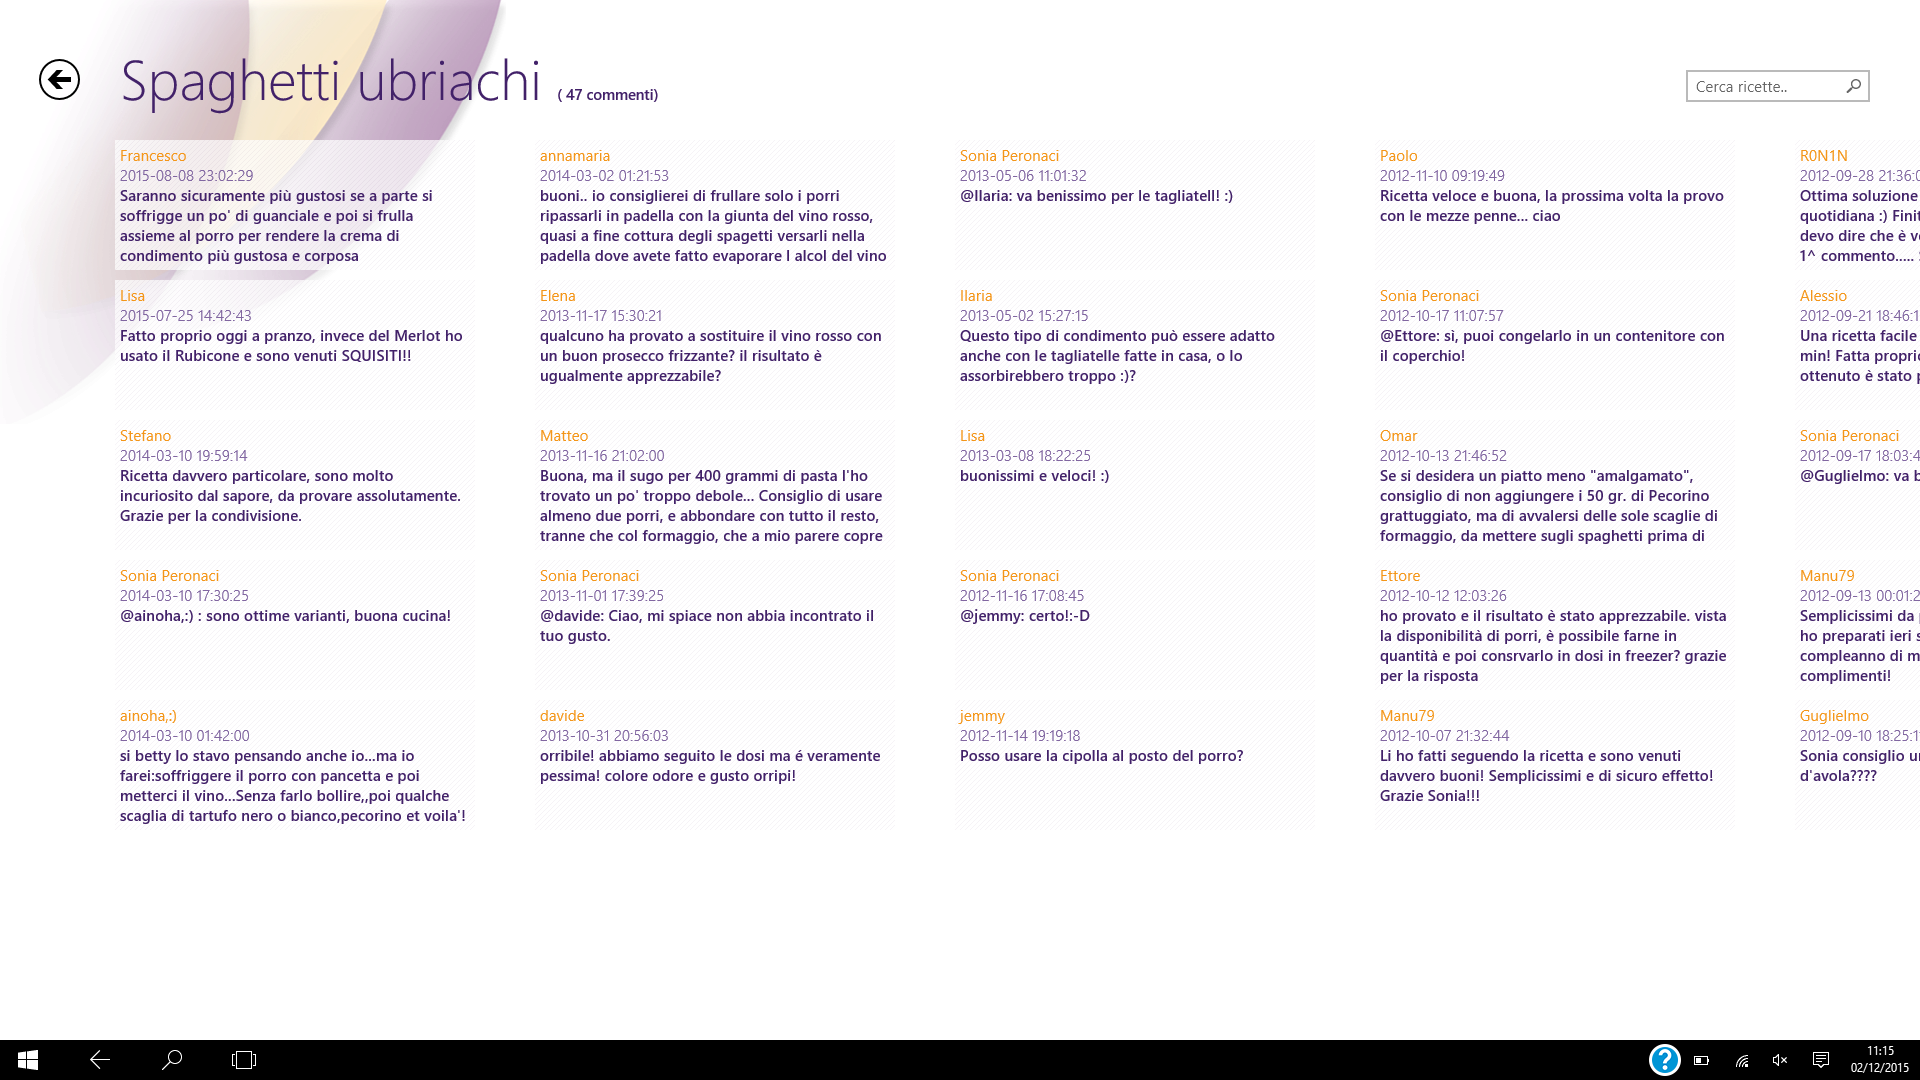
\includegraphics[scale=0.275] {./Giallozafferano/ricetta_commenti.png}  
\captionof{figure}{Schermata commenti\\}
\end{center}

\begin{center}
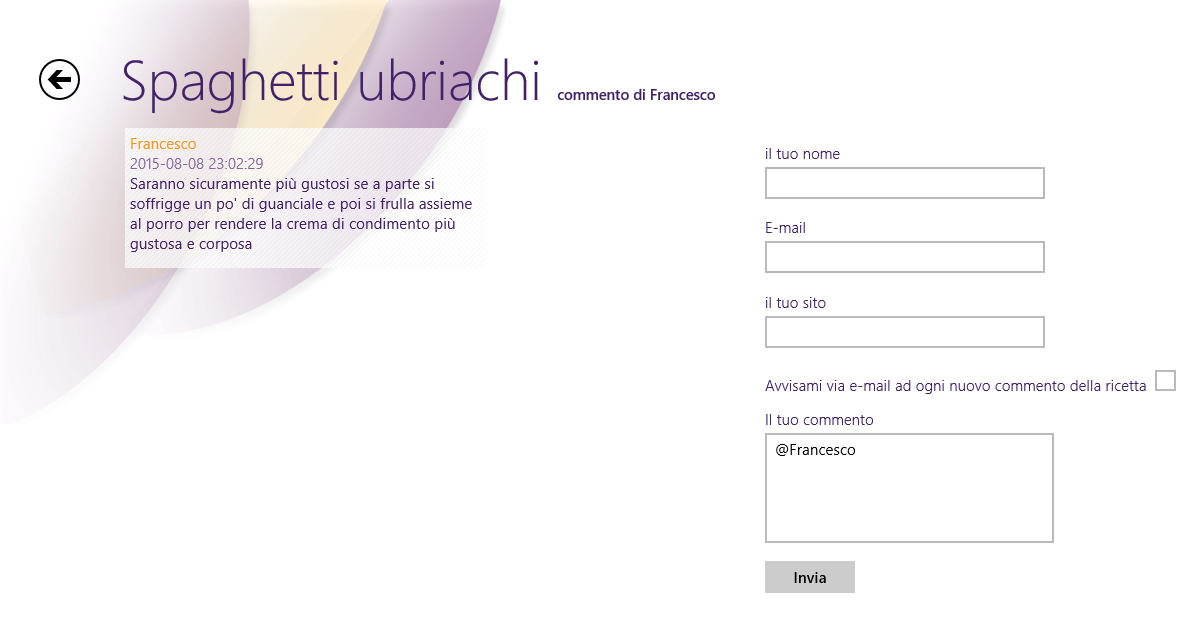
\includegraphics[scale=0.5] {./Giallozafferano/commento_risposta.png}  
\captionof{figure}{Risposta a un commento\\}
\end{center}

Infine la schermata dei preferiti permette facilmente di recuperare ricette salvate precedentemente tra le 3000 proposte.

\begin{center}
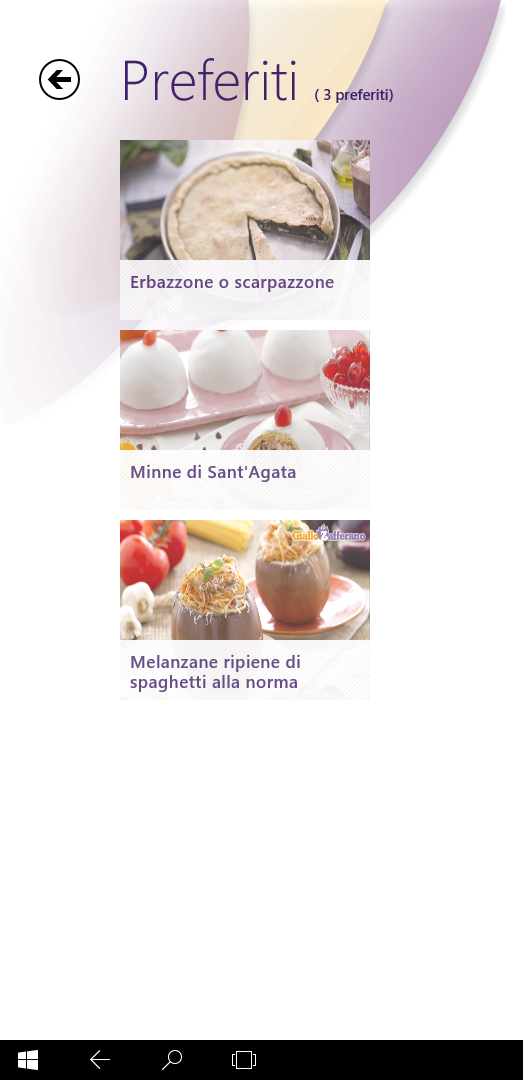
\includegraphics[scale=0.3] {./Giallozafferano/preferiti.png}  
\captionof{figure}{Schermata preferiti\\}
\end{center}

\subsubsection{Allthecooks}
Con oltre 237.000 ricette, Allthecooks è uno dei principale portali culinari internazionali. Ben presente sui social network, offre all'utente un'interfaccia diversa e più funzioni rispetto a GialloZafferano.\\


\begin{center}
\includegraphics[scale=0.275] {./Allthecooks/Home.png}  
\end{center}


\begin{center}
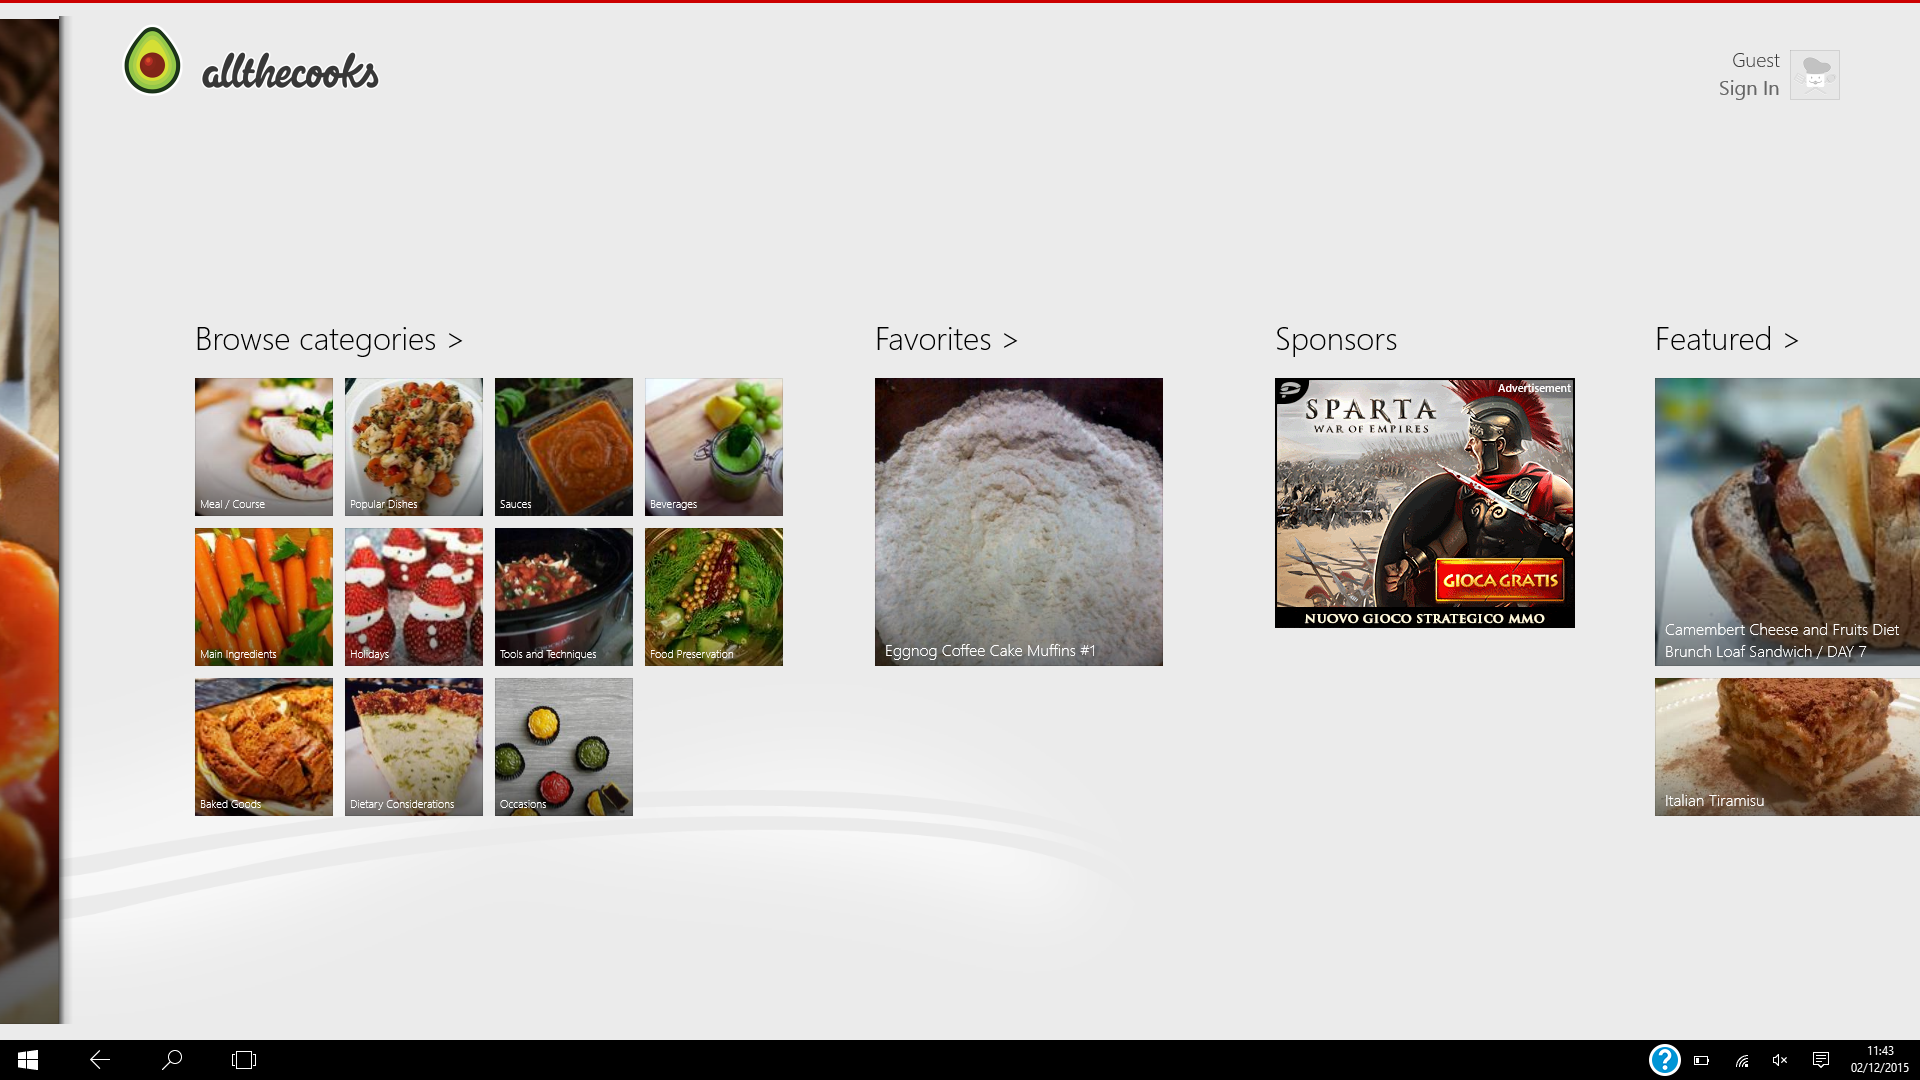
\includegraphics[scale=0.275] {./Allthecooks/home_2.png}  
\captionof{figure}{Schermata principale\\}
\end{center}


\begin{center}
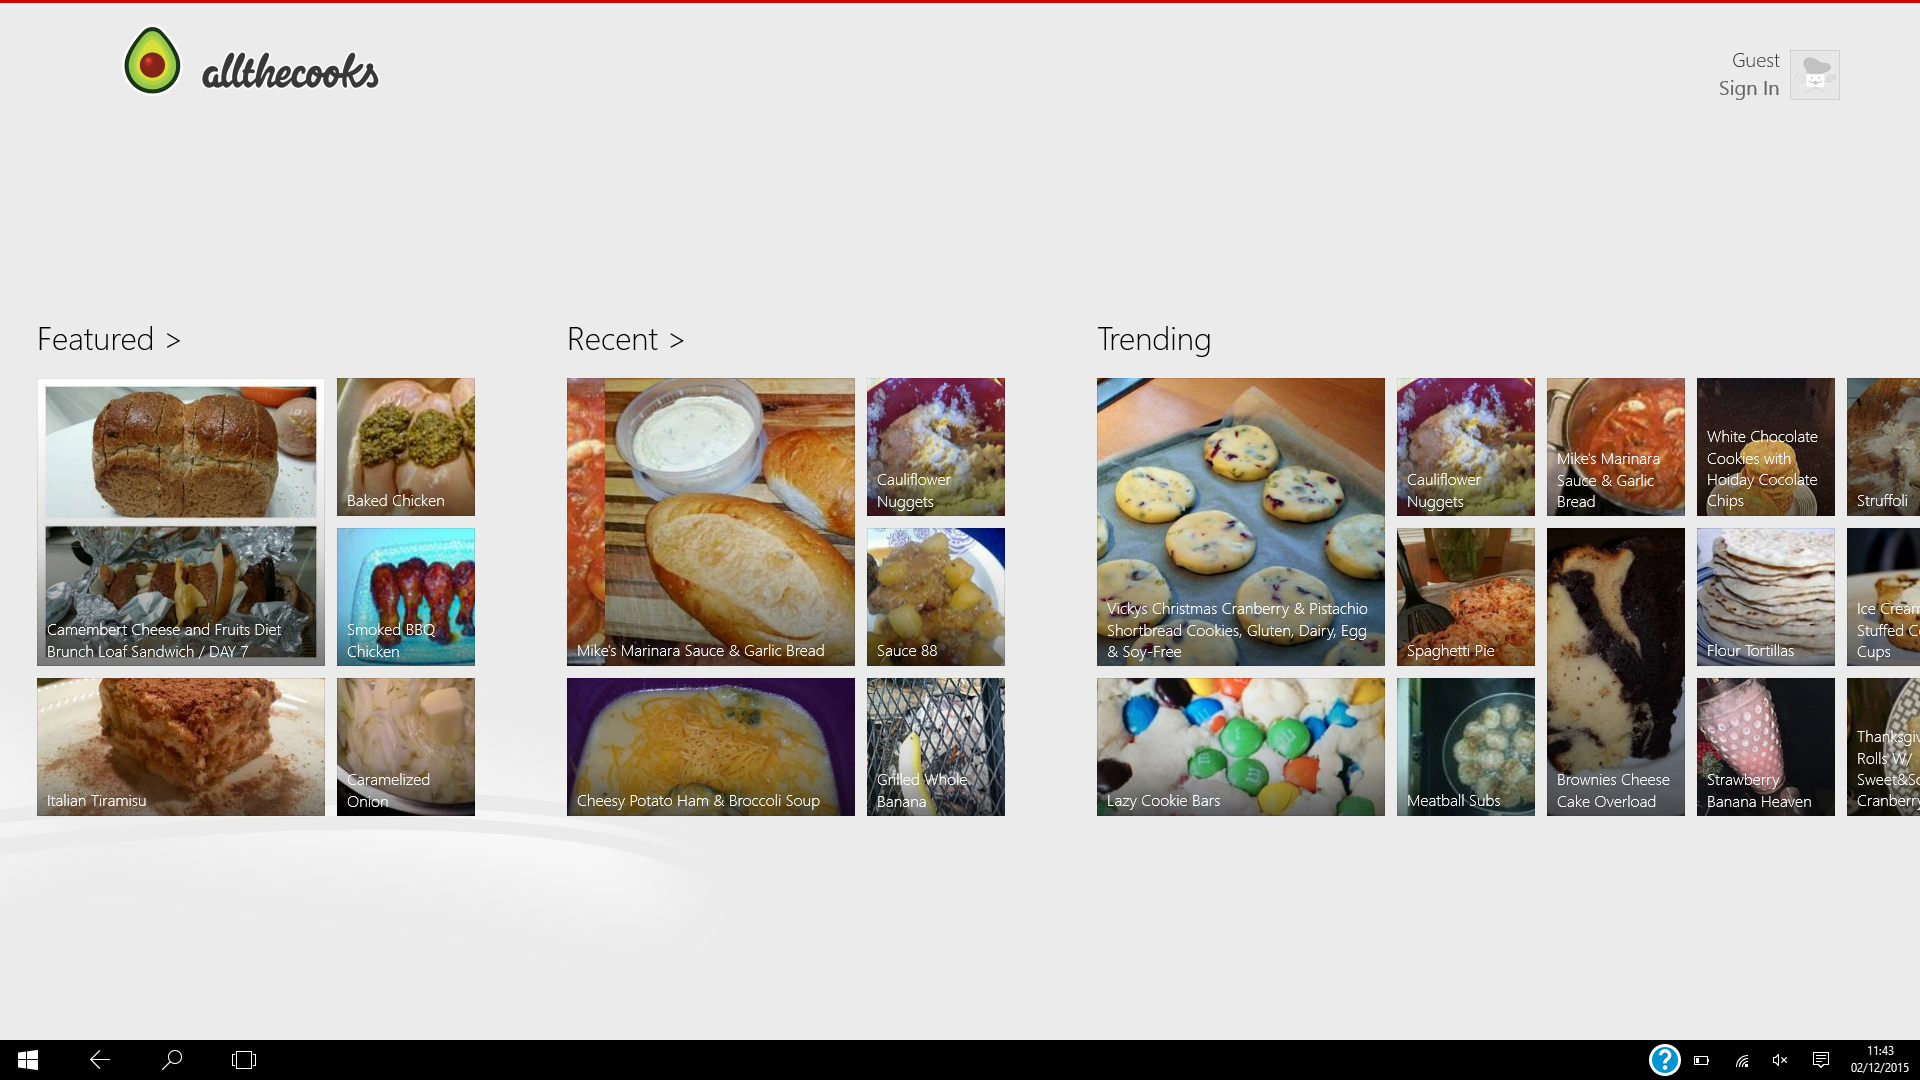
\includegraphics[scale=0.275] {./Allthecooks/home_3.png}  
\captionof{figure}{Schermata principale (scroll orizzontale)\\}
\end{center}

La pagina principale si struttura in orizzontale e prevede un grande slider verticale a sinistra dove vengono visualizzate le ricette più visitate e coerenti con le nostre scelte precedenti.\\
Affianco sono strutturate tutte le sezioni principali come la raccolta delle categorie, le ricette più recenti o quelle più "di moda".\\


\begin{center}
\includegraphics[scale=0.27] {./Allthecooks/categorie.png}  
\captionof{figure}{Schermata categorie (scroll orizzontale)\\}
\end{center}

La schermata principale delle ricette inizialmente mostra tutte le ricette del database, visualizzate a mosaico utilizzando le fotografie caricate dagli autori; inoltre è possibile filtrare i risultati attraverso tag, numero di recensioni/voti e rilevanza.\\


\begin{center}
\includegraphics[scale=0.275] {./Allthecooks/menu.png}  
\captionof{figure}{Schermata categorie con menù\\}
\end{center}

Uno scroll simile a quello già visto per GialloZafferano, visualizza il menù superiore e inferiore insieme.\\
In alto è possibile trovare le funzioni principali legati al profilo (forum, newsletter, notifiche, messaggi e lista della spesa) insieme alla possibilità di tornare alla home o di aggiungere una propria ricetta; in quella inferiore è possibile ricaricare la pagina con un refresh, condividere sui social la pagina in uso o salvare la sezione nei preferiti del sistema operativo.\\


\begin{center}
\includegraphics[scale=0.275] {./Allthecooks/ricetta.png}  
\captionof{figure}{Schermata ricetta (scroll orizzontale)\\}
\end{center}


\begin{center}
\includegraphics[scale=0.275] {./Allthecooks/ricetta_2.png}  
\captionof{figure}{Schermata ricetta (scroll orizzontale)\\}
\end{center}

La schermata distribuisce orizzontalmente tutte le informazioni richieste al momento dell'aggiunta di una ricetta:
\begin{itemize}
\item Un'immagine di copertina, insieme a 5 stelle di voto di apprezzamento
\item Un link al profilo di chi ha aggiunto la ricetta
\item La lista degli ingredienti, automaticamente adattata al numero di porzioni richieste
\item I procedimenti numerati della preparazione
\item Una galleria di fotografie
\item Un'eventuale tabella nutrizionale
\item Una sezione social dove è possibile scegliere dove condividere la ricetta
\end{itemize}

\hspace{-40px}
\begin{minipage}[b]{8.5cm}
	\centering
	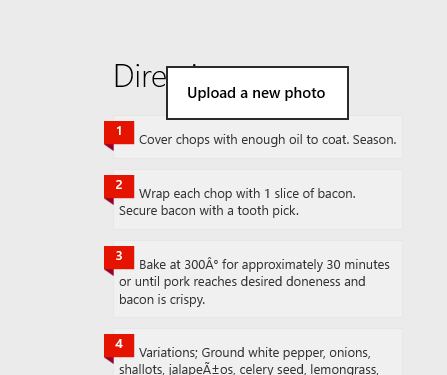
\includegraphics[width=8cm]{./Allthecooks/ricetta_descr_foto.png}
	\captionof{figure}{Add foto al procedimento\\}
\end{minipage}
\ \hspace{2mm}	\hspace{3mm}	\
\begin{minipage}[b]{8.5cm}
	\centering
	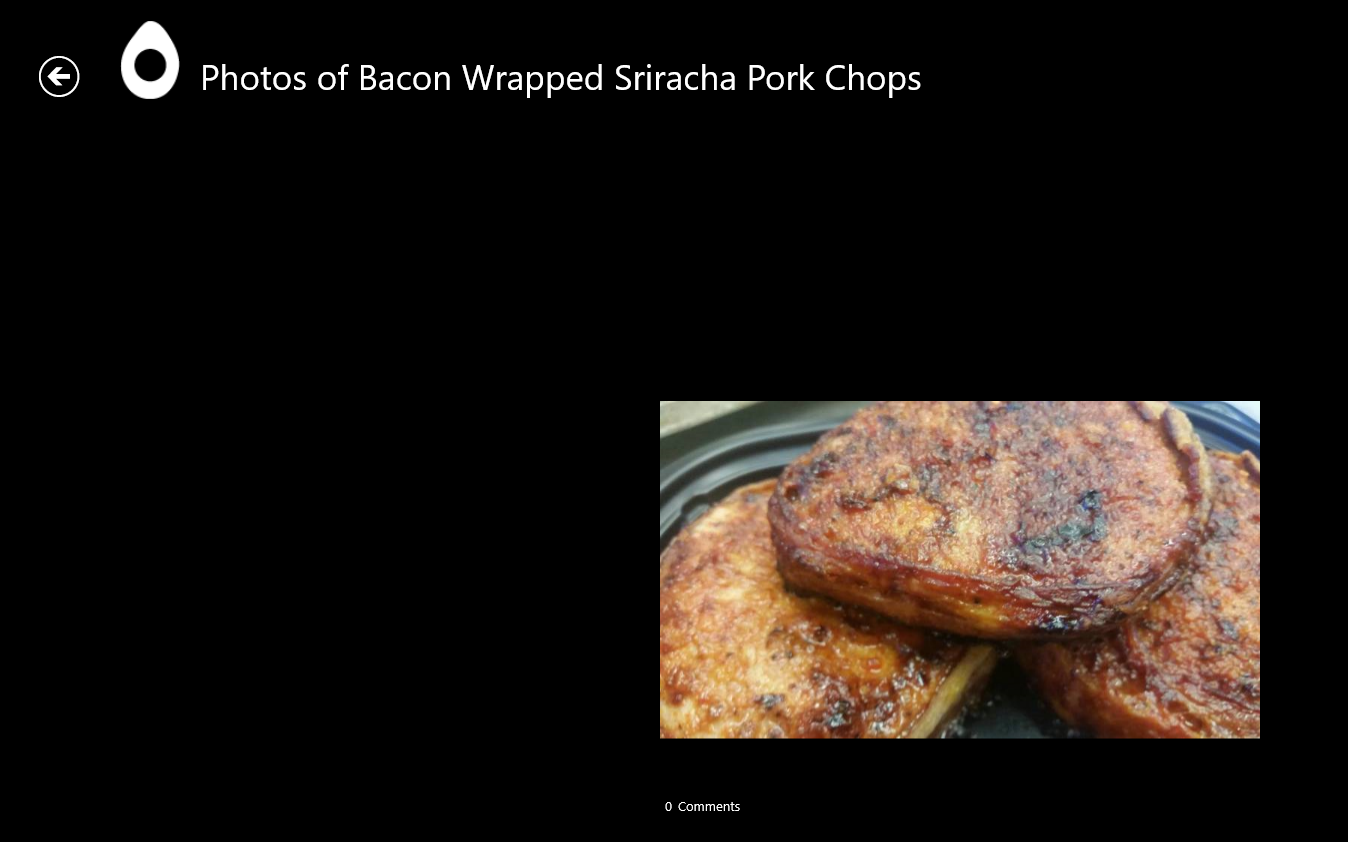
\includegraphics[width=8cm]{./Allthecooks/ricetta_foto.png}
	\captionof{figure}{Schermata galleria ricetta}
\end{minipage}

\begin{center}
\includegraphics[scale=0.27] {./Allthecooks/ricetta_menu.png}  
\captionof{figure}{Schermata ricetta con menù}
\end{center}

Nella schermata ricetta, il menù si arricchisce di nuove funzioni, oltre a quelle già viste:
\begin{itemize}
\item La possibilità di aggiungere la ricetta ai preferiti
\item La possibilità di aggiungere una recensione
\item Si può fare una domanda all'autore
\item Si può aggiungere una fotografia
\item Si possono aggiungere gli ingredienti alla lista della spesa
\item Si può cambiare il sistema metric
\item Si può incrementare la misura del font
\item Stampa della pagina
\end{itemize}


\subsection*{Analisi diretta - Giallozafferano}

\begin{itemize}
\item La schermata principale non occupa interamente lo spazio disponibile e, all'apertura, non vi è un tutorial che ne permetta un veloce apprendimento iniziale. Inoltre non vi è modo di capire che attraverso lo swipe del dito sul margine superiore è possibile visualizzare il menù dell'applicazione.\\ Infine i titoli delle varie sezioni non sono chiaramente cliccabili.

\item Nella pagina di una ricetta, se la difficoltà e/o il tempo di cottura è minimo, la simbologia delle icone non indica adeguatamente il livello, ad esempio 5 salvadanai sbiaditi potrebbero essere confusi con il costo massimo.\\
La lista degli ingredienti è chiaramente visibile, ma non permette di adeguare le porzioni al numero di persone necessarie.\\
Le fotografie non sono ingrandibili, rendendone difficile la visione se il dispositivo in uso è lontano. Non si può condividere la ricetta sui principali social network.\\La sezione delle note è ambigua: non è chiaro se queste note sono personali o pubbliche, vista anche la vicinanza con la sezione dei commenti della community.

\item Non tutte le ricette visualizzano un video esplicativo della preparazione.

\item Non vi è la possibilità di interagire vocalmente con l'applicazione, nè è possibile impostare la grandezza dei testi per facilitare la lettura.

\item Se il menù è visibile, è facile aggiungere gli ingredienti alla lista della spesa. La struttura della pagina "Lista della spesa" è però di difficile uso: è possibile selezionare e spuntare certi ingredienti, ma non è possibile rimuoverli. E' possibile rimuoverli solo attraverso la relativa pagina della ricetta.\\Inoltre se la lista è vuota viene semplicemente visualizzato il titolo senza indicare possibili interazioni o istruzioni.\\
Durante l'uso si sono individuati anche problemi di visualizzazione corretta dei caratteri.

\begin{center}
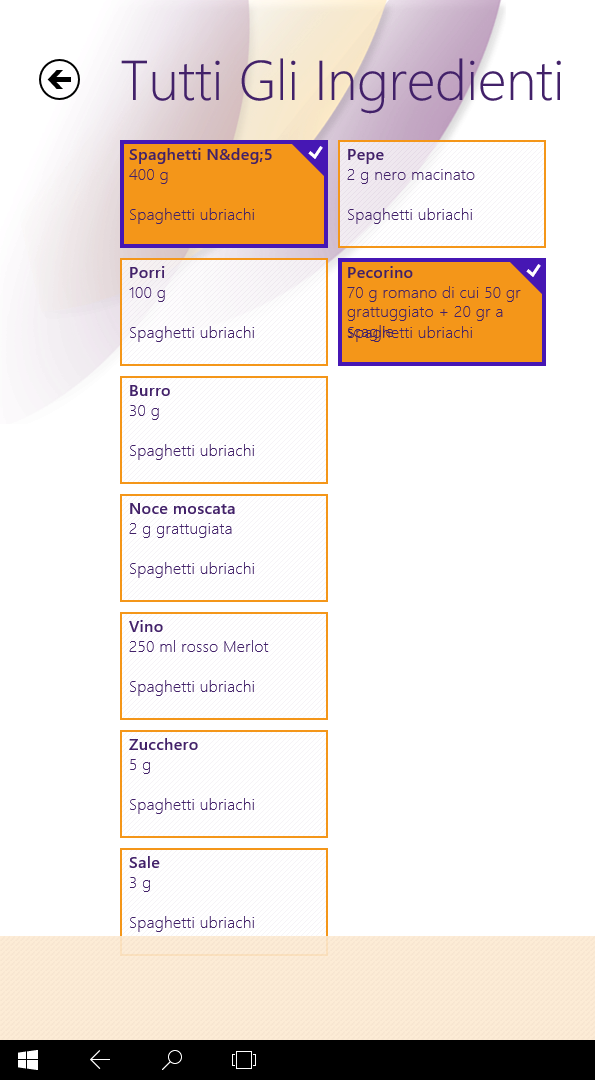
\includegraphics[scale=0.27] {./Giallozafferano/lista_spesa_selezione_1.png}  
\captionof{figure}{Bug visualizzazione caratteri}
\end{center}
\end{itemize}

\subsection*{Analisi diretta - AlltheCooks}

\begin{itemize}
\item La schermata principale occupa interamente lo spazio disponibile ma, all'apertura, non vi è un tutorial che ne permetta un veloce apprendimento iniziale. Inoltre non vi è modo di capire che attraverso lo swipe del dito sul margine superiore è possibile visualizzare il menù dell'applicazione.\\La sezione "panoramica" di sinistra ha lo scroll verticale, ma ci si aspetta di aprire la ricetta cliccando sulla foto, anzichè sul tasto "Learn".\\Non è chiaro che la homepage ha lo scroll orizzontale.

\item Nella pagina di una ricetta, non vi è traccia di indicazioni sul tempo di cottura e difficoltà di preparazione.\\
Vengono mostrate 5 stelle per mostrare il voto alla ricetta, ma non è chiaro come dare un proprio voto.\\
Cliccando su un'istruzione, compare un pop-up per l'inserimento di una fotografia, ma non è chiaro se chiunque può o solo l'autore.\\

\item La barra di ricerca permette l'inserimento di termini, ma l'ok è possibile solo tramite il tasto inivio e non mediante il click sulla lente.

\item Nella ricerca delle ricette, se vengono filtrate per categoria, spesso sono ripetute più volte nei risultati.\\Inoltre è lecito inserire ricette senza fotografie di supporto.

\item L'animazione di caricamento pagina è visualizzata in alto a destra e non è subito visibile e chiara.

\item Quando si aggiunge degli ingredienti alla lista della spesa, non vi è la possibilità di aggiungerli tutti se non selezionandone uno a uno; inoltre nell'apposita pagina non è più presente a quale ricetta facevano riferimento.

\item Nella sezione Forum, il pulsante per inserire una nuova discussione non è di chiara comprensione.

\item L'applicazione permette l'azione "Pin to Start", ma solo cliccandola è chiaro che si riferisce allo Start del sistema operativo.

\end{itemize}

\subsection*{Analisi inversa - Giallozafferano}

A partire dalle 10 euristiche di Nielsen e Molich, individuiamo quali linee guida sono state violate:

\begin{itemize}
\item La linea guida 1 è sicuramente violata dall'errata posizione dell'animazione di loading, poco chiara e poso centrata; inoltre se si accede a una ricetta, l'utente non è informato sul percorso fatto per arrivarci.\\La preparazione della ricetta è più guidata dai numeri sulle immagini che non dal testo che le accompagna.

\item La linea guida 2 è violata nel momento in cui la ricetta è scritta da professionisti: capita spesso che nelle fasi di preparazioni vengano utilizzati termini non adatti a tutti gli utenti. L'applicazione non offre una diversa terminologia a secondo del livello di esperienza impostato dall'utente.

\item Linea guida 3: l'unica interazione possibile dell'utente è nella compilazione di domande/risposte con la community. In questo caso però, nel momento in cui si compila il campo di testo e si torna indietro con l'apposito pulsante, si perderà tutto il contenuto scritto e sarà necessario reinserirlo nuovamente.

\item La linea guida 4 è violata nell'interazione con la community: quando si invia un commento, il sistema non chiede conferma all'utente.

\item La linea guida 5  è violata, data l'assenza di messaggi di errore di qualsiasi tipo. Ad esempio se si tenta di inserire un commento vuoto, il pulsante Invia non notifica nulla.

\item La linea 6 è pesantemente violata dall'assenza di un riferimento al menù, visibile solo mediante lo swipe del margine superiore dello schermo. Non vi è mai una sezione help disponibile.

\item Come già detto nella linea guida 5, l'applicazione non offre nessun tipo di messaggio d'errore. La linea guida 9 è violata.

\item L'applicazione non offre nessun tipo di documentazione o tutorial. La linea guida 10 è violata.
\end{itemize}

\subsection*{Analisi inversa - AlltheCooks}

\begin{itemize}
\item La linea guida 1 è sicuramente violata dall'errata posizione dell'animazione di loading, poco chiara e posizionata in alto a destra; inoltre se si accede a una ricetta, l'utente non è informato sul percorso fatto per arrivarci.\\

\item La linea guida 2 è violata nel momento in cui la ricetta è scritta troppo informalmente: la libertà di inserimento data dall'applicazione non prevede un controllo preliminare dei contenuti aggiunti, quindi il linguaggio familiare si scontra spesso con istruzioni incomplete, a volte addirittura assenti.

\item Linea guida 3: nell'inserimento delle ricette, non è presente una funzione di "redo" una volta abbandonata la finestra. Inoltre se si ricarica la finestra, non viene mostrato il popup di conferma, come viene fatto se si tenta di tornare indietro.

\item La linea guida 4 è violata nell'inserimento delle ricette; ad esempio non vi è una chiara distinzione tra "ingredient" o "ingredient group".

\item La linea guida 5  è violata nell'inserimento delle ricette: ogni errore commesso durante l'input, viene mostrato solo nel riquadro finale e non segnalando il form stesso.

\item La linea 6 è pesantemente violata dall'assenza di un riferimento al menù, visibile solo mediante lo swipe del margine superiore dello schermo. Non vi è mai una sezione help disponibile.

\item La homepage raggruppa molte sezioni, rendendo la grafica confusa e poco minimale. Inoltre la sezione categorie dipende dalle sezioni di filtro, piuttosto che da categorie preimpostate. E' violata la linea guida 8.

\item L'applicazione non offre nessun tipo di documentazione o tutorial. La linea guida 10 è violata.
\end{itemize}






\end{document}
\section{Studio di fattibilità}

\subsection{Contesto d'uso}
Dalle analisi precedenti di user research e valutazione di sistemi
esistenti si può fare un quadro del contesto d'uso dell'applicazione
proposta.
Vedremo in particolare qual'è il target d'utenza, quali sono i task da
prendere in considerazione e quali sono i possibili vincoli tecnici e
ambientali.

\subsubsection{Target d'utenza}
Come emerge dalla user research il target d'utenza previsto è molto
eterogeneo, infatti non si sono riscontrati dei restrittivi limiti di
età, istruzione o competenze culinarie.\\
Forse l'unica vera restrizione riguarda la nazionalità degli utenti
in quanto si è deciso di concentrare
l'attenzione verso l'utenza italiana. Questa scelta è nata dall'analisi
delle statistiche le quali suggeriscono che l'Italia è una delle
prime nazioni nel mondo per quanto riguarda la passione culinaria
\ref{fig:cooking-country}. A conoscenza di ciò, focalizzarsi su un
utenza internazionale avrebbe potuto confondere gli italiani, poco familiari
con lo stile culinario non tradizionale. Ad esempio la colazione
italiana prevede un pasto molto rapido a differenza di molte colazioni
estere e la suddivisione delle portate in ``primo'' e ``secondo'', le quali
identificano già la categoria della pietanza, non è molto comune
all'estero.

\subsubsection{Task}
A seguito delle valutazioni dei sistemi esistenti, è risultato opportuno
rivisitare la lista dei task già definita nello user research
\ref{tasks}, con
l'idea di far forza sul contesto nel quale le applicazioni esistenti
mostrano le loro debolezze.

\begin{enumerate}
\label{tasks}

\item Impostare il livello di preparazione culinaria
\item Accedere alla documentazione/help dell'applicazione

\item Ricerca di una ricetta per nome.
\item Ricerca di una ricetta per ingredienti.

\item Ricerca di una ricetta sfogliando le categorie.

\item Filtro di una ricerca in base agli ingredienti.
\item Filtro di una ricerca in base alle intolleranze/allergie/diete.

\item Individuare la difficoltà di preparazione e il costo di una ricetta.
\item Individuare gli ingredienti necessari alla preparazione di una ricetta.
\item Distinguere le varie fasi di una preparazione della ricetta.
\item Distinguere la vista passo-passo della preparazione dalla visione complessiva della ricetta.
\item Visionare un video di presentazione della ricetta
\item Condividere una ricetta sui social network.
\item Creare un menù completo selezionando una lista di ricette.
\item Aggiungere/Rimuovere una ricetta al menù già creato.
\item Cercare un menù consigliato da CookApp.

\item Inserire una nuova ricetta nel database dell'applicazione.
\item Interagire con la community rispondendo a problemi degli utenti.
\item Chiedere consiglio alla community creando un nuovo topic.
\item Chiedere aiuto "live" alla community riguardo un particolare passaggio della ricetta oppure riguardo agli ingredienti

\item Salvare/Rimuovere una ricetta nei preferiti.
\item Salvare/Rimuovere un menù nei preferiti.

\item Accedere alla lista della spesa.
\item Inserire/Rimuovere gli ingredienti di una ricetta nella lista della spesa.
\item Inserire/Rimuovere gli ingredienti di un menù nella lista della spesa.

\item Votare e commentare le ricette ed i menu.

\item Mandare una richiesta di pronto intervento a tutti i gli amici per chiedere loro se in casa hanno un ingrediente e se possono aiutare.

\item Visualizzare il progresso della preparazione del menù e della singola ricetta



\item Trova i punti vendita degli ingredienti della lista della spesa.
\item Interagire con la mappa del percorso mediante lo smartwatch per strada e nel punto vendita.
\item Identificare il prodotto acquistato con l'NFC dello smartwatch eliminando la relativa voce dalla lista della spesa.
\item Aggiungere/confermare una voce nella lista della spesa con lo smartwatch.


\item Avanzare con le fasi di preparazione passo-passo mediante messaggi vocali.
\item Text-to-Speech delle fasi di preparazione di una ricetta.


\end{enumerate}

Vedremo in seguito gli approcci delle applicazioni già esistenti verso
questi task e le funzionalità da progettare nella nostra applicazione
affinché tali task possano essere eseguiti al meglio.


\subsubsection{Vincoli tecnici ed ambientali}
L'applicazione è pensata per essere utilizzata in ambienti probabilmente
molto caotici, in cui l'attenzione dell'utente potrebbe essere
facilmente catturata da altri elementi del contesto. Questo aspetto è
stato riscontrato anche durante le osservazioni del contextual inquiry:
i tre studenti si sono facilmente distratti a causa dell'euforia della
novità, mentre la signora Antonietta si è fatta distrarre dalla
discussione con la sorella. A rafforzare tale supposizione sono i
risultati del sondaggio i quali mostrano che il livello di esperienza
culinaria media è medio-bassa.
Un vincolo per l'appliczione
potrebbe essere infatti la disposizione disordinata degli ingredienti
e degli atrezzi nella cucina, che potrebbe impediere un comodo
raggiungimento e utilizzo del
device, scoraggiando l'utente all'approccio tecnologico. Inoltre
avere le mani impegnate potrebbere rendere l'applicazione inutilizzabile
in alcuni casi, soprattuto se l'ausilio dei comandi vocali non fosse
previsto. Ad ogni modo anche nche nel caso in cui fossero previsto comandi vocali,
un ambiente molto caotico potrebbe essere un vincolo.\\
Il tutto suggerisce di progettare un applicazione la cui interfaccia sia
molto semplice, immediata e che riduca il carico di stress
percepito dall'utente.

\subsection{Personas}
\begin{table}[H]
	\begin{centering}
	\begin{tabular} { | r  p{10cm} | }
		\hline
		\multirow{2}{*}{
			\begin{minipage}{.18 \textheight}
				\vspace{0.1in}
				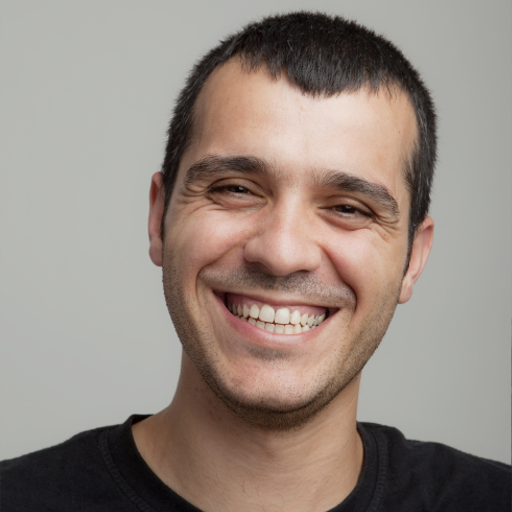
\includegraphics[width=\linewidth]{img/personas/filippo.png}
			\end{minipage}
		}
		 & \vspace{0.1 in}\Large\textbf{Filippo} \\ 
		& \vspace{0.1 in}\large{\emph{``Anche se viaggio molto per catturare il mondo,
cucinare all'estero mi fa
		sentire sempre a casa. Sempre pronto a re-inventare la tradizione anche con
		ingredienti difficili.''}}\\[8ex] 
		\hline
		\textbf{Anni} & 36 \\ \hline
		\textbf{Occupazione} & Fotografo \\ \hline
		\textbf{Famiglia} & {Nonostante i frequenti viaggi, ha uno
studio e un domicilio a Rimini, città in cui è cresciuto con la sua
famiglia. Ogni circa due settimane Filippo fa visita ai genitori per il
pranzo domenicale insieme alla sua ragazza spagnola con cui convive.} \\
\hline
		\textbf{Profilo Tecnico} & Dopo il liceo artistico ha vissuto 5
anni in Spagna, lavorando sia come cameriere in un ristorante italiano
sia come impiegato in un'agenzia di viaggi. Tornato in italia ha poi
deciso di seguire la sua passione per la fotografia iscrivendosi
all'accademia delle belle arti. Terminati gli studi ha iniziato a
viaggiare in tutto il mondo pubblicando le sue foto in un blog wordpress gestito
da lui stesso. Da 2 anni ha aperto un proprio studio fotografico in
Italia. \\ \hline
		\textbf{Hobby} & Ha sempre avuto una grande passione per il
rugby, sport che ha abbandonato dopo l'università anche se continua a
seguirlo assiduamente. \\ \hline
		\textbf{Rapporto con la cucina} & Nonostante gli piaccia molto
la cucina spagnola e quella asiatica, rimane molto legato alla cucina
tradizionale italiana. Cucina spesso e volentieri piatti italiani molto
semplici ma che comunque sono molto graditi dalla sua ragazza spagnola.
\\ \hline
		\textbf{Rapporto con la tecnologia} & Prima di quest'anno non
aveva mai considerato
l'acquisto di un tablet, essendo abituato a lavorare sempre il laptop 
per necessità di utilizzo di software di editing
d'immagini. Dopo avero provato un tablet surface, che permette di
passare in modalità desktop agganciando una tastiera al dispositivo, ha
deciso di comprarne uno, affascinato dalla possibilità di poter
continuare ad utilizzare i suoi software con interfaccia destkop e
sfruttare allo stesso tempo l'estrema mobilità e le app di un tablet.
Ha anche una buona familiarità con il Web avendo gestito in passato un proprio
blog di foto ed una pagina facebook. Lo scorso natale la ragazza gli ha
regalato uno smartwatch che inizialmente non trovava di particolare
utilità, ma dopo aver visto che gli permette di visualizzare a distanza
la ripresa della fotocamera del suo smartphone ha iniziato ad
utilizzarlo regolarmente come supporto alla fotografia. Infatti ha
intenzione di acquistare prossimamente una nuova reflex con sistema
operativo Android da integrare al suo smartwatch.
\\ \hline
	\end{tabular}
	\end{centering}
\end{table}


\begin{table}[H]
	\begin{centering}
	\begin{tabular} { | r  p{10cm} | }
		\hline
		\multirow{2}{*}{
			\begin{minipage}{.18 \textheight}
				\vspace{0.1in}
				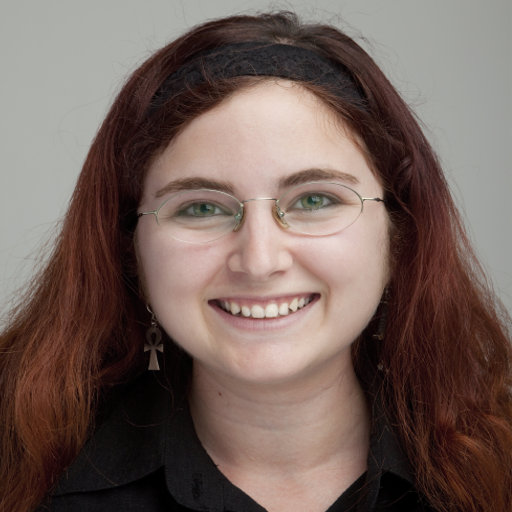
\includegraphics[width=\linewidth]{img/personas/flora.png}
			\end{minipage}
		}
		 & \vspace{0.1 in}\Large\textbf{Flora} \\ 
		& \vspace{0.1 in}\large{\emph{``I love dogs as much as I
love Italian guys. They are all handsome and funny and I am trying to
	lose some weight to look prettier. Maybe some of them will notice
me.''}}\\[8ex] 
		\hline
		\textbf{Anni} & 28 \\ \hline
		\textbf{Occupazione} & Dottoranda in geologia \\ \hline
		\textbf{Famiglia} & {Ha vissuto a Glasgow in Scozia con la madre
ed il fratello maggiore fino ai tempi del liceo. Si è poi trasferita in
un campus ad
Edimburgo per frequentare l'università. Data la breve distanza tra le
due città non ha sofferto il distacco dalla famiglia tornando a casa
quasi ogni fine-settimana. Da due anni ha lasciato la Scozia e le manca molto il
fratello con cui ha un rapporto molto speciale maturato dopo il
divorzio dei genitori.} \\
\hline
		\textbf{Profilo Tecnico} & Si è specializzata in geologia presso
l'università di Edimburgo. Ha ottenuto poi una borsa di studio per un
dottorato di ricerca all'Università di Bologna. Non ha mai lavorato al
di fuori dell'ambito accademico.\\ \hline
		\textbf{Hobby} & Ama i cani e prendersi cura di loro. Nel
fine-settimana lavora occasionalmente come dog-sitter, non molto per
bisogni economici ma per passare un po' di tempo con i cani visto che ha
dovuto lasciare il suo terrier in Scozia. \\\hline
		\textbf{Rapporto con la cucina} & Come tutti gli scozzesi ama
la cucina italiana, in particolare il gelato e la lasagna. Nei
primi mesi di dottorando in Italia ha messo su qualche chilo e ha deciso
quindi di iniziare una dieta. Spesso però, soprattuto nei periodi dalle
scadenze accademiche, non riesce a resistere ad una buona pizza o alla
trattoria bolognese,
sia per dare sfogo allo stress, sia per l'impegno di fare spesa e
cucinare.\\ \hline
		\textbf{Rapporto con la tecnologia} & Utilizza quotidianamente
il PC per fare ricerca e lo smartphone per messaggiare con gli amici.
Quando è a casa predilige il tablet perchè spesso effettua lunghe
videochiamate con la madre con cui comunica anche durante lo svolgimento
di altre mansioni, spostandosi da una stanza all'altra.\\ \hline
		\textbf{Altri particolari} & Condivide un appartamento con altri
due studenti molto più piccoli di lei. Periodicamente organizzano feste
in casa anche infrasettimanalmente. Lei ormai stanca delle feste
universitarie che si prolungano fino a tarda notte, si fa spesso ospitare
dall'amica Francesca in queste occassioni. Anche se prova una sorta di disagio per il
disturbo creato all'amica, ritiene sia l'unico modo per affrontare la giornata
succesiva.\\ \hline
	\end{tabular}
	\end{centering}
\end{table}

\begin{table}[H]
	\begin{centering}
	\begin{tabular} { | r  p{10cm} | }
		\hline
		\multirow{2}{*}{
			\begin{minipage}{.18 \textheight}
				\vspace{0.1in}
				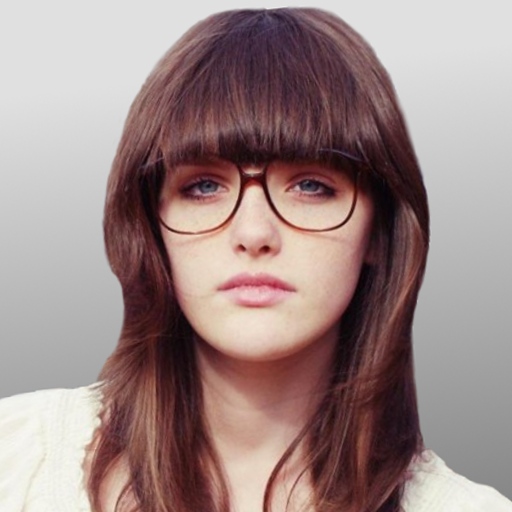
\includegraphics[width=\linewidth]{img/personas/francesca.png}
			\end{minipage}
		}
	 	& \vspace{0.1 in}\Large\textbf{Francesca} \\ 
		& \vspace{0.1 in}\large{\emph{``Ho una gran passione per l'indie rock e
il vintage design. Da due anni ho deciso di diventare vegetariana, sia
per rispettare la mia salute sia per contrastare lo sfruttamento animale
delle multinazionali.''}}\\[8ex] 
		\hline
		\textbf{Anni} & 27 \\ \hline
		\textbf{Occupazione} & Giornalista tirocinante \\ \hline
		\textbf{Famiglia} & È figlia unica ed è stata cresciuta 
a Verona dai genitori, che le hanno permesso sempre di inseguire le sue
passioni.\\ \hline
		\textbf{Profilo Tecnico} & Dopo aver terminato il liceo classico
di Verona, si è trasferita a Bologna per frequentare l'università.
Laureata da un anno in lettere e filosofia ha iniziato da qualche mese
un tirocinio retribuito in una nota testata giornalistica a Bologna. \\\hline
		\textbf{Hobby} & Nel tempo libero le piace cucire sciarpe e
capelli per lei e per il suo ragazzo. Il finesettimana non perde mai un
concerto indie rock e frequenta spesso i negozi dell'usato per alla
ricerca di oggettistica vintage. \\ \hline
		\textbf{Rapporto con la cucina} & È diventata vegeteriana dopo
aver lasciato Verona. Il suo cambio di alimentazione non è stato
drastico in quanto non le è mai piaciuta molto la carne. Il problema le
si presenta quando mangia fuori casa con altre persone, occasioni in cui
prestare attenzione agli ingredienti delle pietanze che mangia. \\ \hline
		\textbf{Rapporto con la tecnologia} & Si è sempre definita
riluttante alla tecnologia, prediligendo canali d'informazione più
classici rispetto al web. Ha utilizzato il PC per lunghi periodi
solamente per scrivere le sue tesi universitarie. Non possiede uno
smartphone e continua ancora ad utilizzare gli SMS.\\ \hline
		\textbf{Altri particolari} & Frequenta da pochi mesi un ragazzo
amante di cucina tipica emiliana. Nonostante i loro tipi di
alimentazione molto diversi, il cibo non è mai una causa di discussione. \\\hline
	\end{tabular}
	\end{centering}
\end{table}

\begin{table}[H]
	\begin{centering}
	\begin{tabular} { | r  p{10cm} | }
		\hline
		\multirow{2}{*}{
			\begin{minipage}{.18 \textheight}
				\vspace{0.1in}
				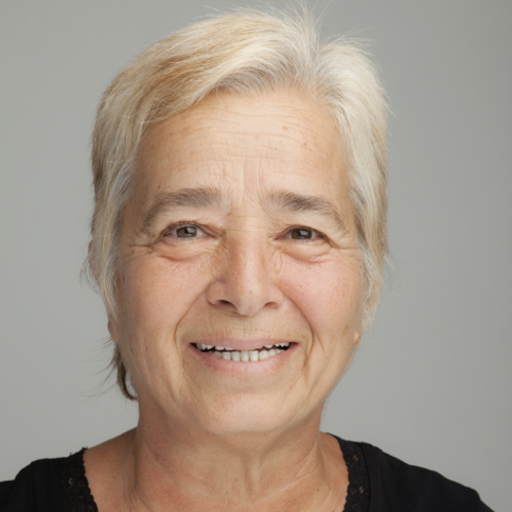
\includegraphics[width=\linewidth]{img/personas/maria.png}
			\end{minipage}
		}
	 	& \vspace{0.1 in}\Large\textbf{Maria} \\ 
		& \vspace{0.1 in}\large{\emph{``I miei figli vivono tutti in
città, ma io la montagna proprio non la lascio. Qui l'aria è buona e si
mangia bene, altro che i faste fud dove vanno i miei nipoti. Almeno con
il nuovo tablet che mi hanno regalato li vedo spesso con l'internet.''}}\\[8ex] 
		\hline
		\textbf{Anni} & 63 \\ \hline
		\textbf{Occupazione} & Pensionata \\ \hline
		\textbf{Famiglia} & Ha due figli maschi ed una femmina. I due
maschi vivono entrambi a Milano mentre la figlia vive a Napoli dopo
essersi sposata con un carabiniere conosciuto durante un suo periodo di servizio a
Milano. Quasi una volta al mese i figli di Milano vanno a trovarla a
Cusio, un piccolo paesino di montagna in provincia di Bergamo dove
tutt'ora vive. La signora Maria però, soffre molto la distanza con
l'altra figlia che riesce a vedere solo una volta l'anno durante le
feste natalizie. \\ \hline
		\textbf{Profilo Tecnico} & Ha lavorato per tutta la vita come
postina a Cusio e nei dintorni. Adesso si gode una meritata pensione. \\ \hline
		\textbf{Hobby} & Ha sempre avuto la passione per il ballo, che
coltiva con suo marito frequentando occasionalmente la balera del paese.
Oltre al liscio ha una vera ossessione per le telenovelas e tutti i
programmi TV condotti da Maria De Filippi.  \\\hline
		\textbf{Rapporto con la cucina} & A detta dei nipotini, abituati
alla cucina di città, la nonna Maria è la cuoca
più brava del mondo. Abituata ad una cucina molto tradizionale e
montana, il suo piatto forte sono i fagottini con funghi porcini e
Bitto, un formaggio di mucca tipico della Lombardia. Purtroppo il
marito della figlia che vive a Napoli è intollerante al lattosio e
quando c'è anche lui a tavola questo piatto diventa un tabù.\\ \hline
		\textbf{Rapporto con la tecnologia} & Non ha mai utilizzato un
computer. Per molto tempo i figli milanesi hanno cercato di farle
utilizzare uno
smartphone ma con scarso successo in quanto Maria, a causa
dell'abbassamento della vista, ha riscontrato che si stanca molto
	durante l'interazione con i piccoli schermi degli smartphone. I
figli hanno deciso quindi di regalarle un tablet in quanto ha uno schermo più
grande rispetto agli smartphone e molte applicazioni pensate appositamente per gli anziani.
Alla signora Maria sembra piaciere il nuovo dispositivo e, nonostante abbia dei 
tempi molto lenti di apprendimento, è molto motivata ad
imparare come utilizzarlo in quanto le permette di
videochiamare la figlia che vive a Napoli e vedere le foto dei nipotini
mentre crescono. \\ \hline
		\textbf{Altri particolari} & Il marito della signora Maria è
molto orgoglioso delle sue origini nordiche e non ha mai preso in
simpatia il carabiniere napoletano che la figlia ha sposato. \\\hline

	\end{tabular}
	\end{centering}
\end{table}

\begin{table}[H]
	\begin{centering}
	\begin{tabular} { | r  p{10cm} | }
		\hline
		\multirow{2}{*}{
			\begin{minipage}{.18 \textheight}
				\vspace{0.1in}
				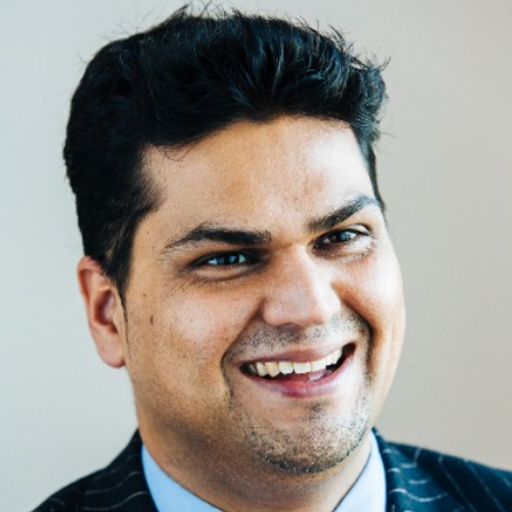
\includegraphics[width=\linewidth]{img/personas/giuseppe.png}
			\end{minipage}
		}
	 	& \vspace{0.1 in}\Large\textbf{Giuseppe} \\ 
		& \vspace{0.1 in}\large{\emph{``I milanesi parlano tutti male di
Napoli, ma dopo esserci stati non se ne vogliono più andare. Mia moglie
milanese infatti adesso ama la mia città tanto quanto ama me. Solo noi abbiamo il
sole, il mare, la pizza e il babà.''}}\\[8ex]
		\hline
		\textbf{Anni} & 42 \\ \hline
		\textbf{Occupazione} & Maresciallo dei Carabinieri \\ \hline
		\textbf{Famiglia} & Ha sposato Chiara, una donna del nord
Italia, conosciuta durante un periodo di servizio a Milano. Hanno una
bambina di 6 anni.\\ \hline
		\textbf{Profilo Tecnico} & Dopo le scuole superiori si
arruola all'Accademia Militare per intraprendere gli studi in
Giurisprudenza e diventare un ufficiale. Viene in seguito reclutato come
maresciallo dell'Arma dei Carabinieri. Attualmente è in comando stabile
presso una caserma della periferia di Napoli. \\\hline
		\textbf{Hobby} & Fuori servizio, quando non passa del tempo con
la sua famiglia, pratica il tiro con l'arco.\\ \hline
		\textbf{Rapporto con la cucina} & È di buona forchetta e gli
piace molto cucinare. Ha una buona esperienza con i fornelli maturata
durante il periodo dell'Accademia Militare e ama i piatti tipici
Napoletani e gli ingredienti del sud Italia. Negli ultimi anni però il
medico gli ha proibito di consumare latticini a causa di un intolleranza al
lattosio. Giuseppe ha impiegato diverso tempo per accettare la sua
intolleranza avendo avuto sempre un debole per la mozzarella di bufala.\\ \hline
		\textbf{Rapporto con la tecnologia} & Utilizza il PC in caserma
esclusivamente tramite il sistema software dei Carabinieri per risolvere
le pratiche quotidiane. A casa utilizza sporadicamente il
laptop della moglie giusto per navigare e riprodurre video. Possiede uno
smartphone ma lo utilizza principalmente per le classiche telefonate e fotografare i
piatti ai ristoranti.\\ \hline
	\end{tabular}
	\end{centering}
\end{table}
\subsection{Scenari d'uso}
\begin{enumerate}

\item Filippo nell'ultimo viaggio in brasile ha conosciuto Paulo, un
impiegato in banca appassionato di fotografia. Filippo ospiterà per un
weekend Paulo
e suoi 3 amici che stanno visitando l'Italia. A tal proposito voleva
preparare una cena tipica italiana di benvuto. Per non risultare banale,
si affida a
CookApp scegliendo uno tra i menù preimpostati consigliatii. Il menù
scelto prevede per antipasto ``Capasanta atlantica con gatzpacho fresco
e croccante di pane'', per primo dei ``Ravioletti ripieni di cacio e
pepe'' e per secondo una ``tagliata di fassona piemontese''. Decide però
di sostituire il secondo con ``Spiedini di gamberi'', un piatto scelto tra i ``Tipici della
zona''. Infine come dolce, inserisce un classico ``Tiramisù'' nel menù.
Dopo aver ultimato le modifiche al menù aggiunge tutti gli ingredienti
necessari alla lista della spesa. Dalla schermata della lista della
spesa Filippo cerca i punti vendita dove per poter acquistare gli
ingredienti e scegli quelli più vicino a casa. A questo punto esce di
casa seguendo il percorso verso i punti vendita selezionati,
visualizzati sulla mappa del suo smartwatch. Arrivato al primo punto
vendita lo smartwatch indica, tramite una mappa più dettagliata, le posizioni degli ingredienti delle
relative corsie del supermercato. Grazie al modulo NFC dello smartwatch,
Filippo scansiona il tag NFC dei prodotti da acquistare che vengono
automaticamente confermati sulla lista della spesa. Infine si dirige
alla cassa e effettua il pagamento di tutta la spesa posizionando lo
smartwatch al sensore della cassiera. 
Finita la spesa nei diversi punti vendita, Filippo torna a casa e
prepara una deliziosa cenetta per i suoi amici brasiliani.


\item Per le vacanze di Pasqua i coinquilini di Flora tornano a casa dalla famiglia, e
lei decide quindi di invitare per pranzo l'amica Francesca e il suo
ragazzo Enrico, per voler ricambiare la grande ospitalità che lei spesso
le offre. Flora vorrebbe realizzare un menù tipico Pasquale ma
solitamente era sempre tornata in Scozia per le vacanze e non ha idea di
cosa mangino gli italiani in queste occasioni.

Tramite l'applicazione
cookApp, già impostata in lingua inglese grazie al riconoscimento della lingua
di sistema del suo tablet, Flora accede alla categoria ``Holidays'' e alla
sottocategoria ``Easter'' trovando facilmente i piatti tipici pasquali. 
Si ricorda però che la sua amica Francesca è vegetariana quindi
seleziona il filtro di vista ``With vegetarian version'' che le permette
di visualizzare tutte le ricette che abbiano anche le istruzioni per
prepararne una variante vegetariana. Ha preferito questo filtro rispetto
a ``Vegetarian'' in quanto il ragazzo di Francesca è amante della carne e
così ha modo di prepare gli stessi piatti per tutti, ma in due versioni
diverse. Una volta individuate le ricette decide di aggiungerle ad un
nuovo menù personalizzato. CookApp inoltre, durante la consultazione
della categoria pasqua, suggerisce a Flora di decorare la
tavola con degli ovetti di pasqua, che all'apparenza sembrano delle
classiche uova sode decorative ma che poi riveleranno una simpatica sorpresa al
loro interno. Grazie a CookApp Flora riesce a preperare senza difficoltà
il pranzo pasquale a fare felici i suoi amici.


\item La signora Maria, in occasione della visita che le faranno
l'indomani i suoi figli da Milano, decide di preparare i fagottini al
Bitto che tanto piacciono al suo nipotino Marco. La mattina dopo Chiara, la
figlia di Maria che vive a Napoli, avverte sua madre che è in viaggio,
insieme a suo marito carabiniere Giuseppe e la loro bambina,
per andare a trovarla. Le dice anche che arriverrano per l'ora di pranzo, scusandosi
per non averglielo detto prima ma si sono
riusciti ad organizzare solamente all'ultimo momento. Maria è molto
felice che si riunirà tutta la famiglia anche se è un po' dispiaciuta
perchè non può più prepare i fagottini al Bitto inquanto Giuseppe è
intollerante al lattosio. Inoltre la decisione di Maria
altera l'animo del marito il quale sostiene che il carabiniere non è
davvero intollerante ma ha problemi con le mozzarelle napoletane perchè
contaminate dai rifiuti del sottosuolo campano. Non volendo far
dispiacere nessuno, la signora Maria prova a cercare su CookApp una
variante dei fagottini al Bitto per intolleranti al lattosio. In
particolare scrive ``fagottini al bitto'' nella barra di ricerca
selezionando il filtro ``Senza lattosio''. Non ottiene nessun risultato
ma CoockApp le chede se vuole rivolgersi alla comunità online per un
aiuto sulla ricetta ``Fagottini al bitto''. Maria pigia l'apposito
pulsante di conferma e tramite la casella di inserimento e il pulsante
di invio, pubblica la sua richiesta per la community. Ottiene nel giro
di qualche minuto una risposta di una ragazza di Sondrio che le
consiglia di utilizzare un composto di maionese e tofu. Maria seleziona
quest'ultimo ingrediente e ne compare una descrizione, oltre ad un
pulsante ``Dove comprare''. Maria lo pigia e compare una mappa di
supermercati nelle vicinanze. Nota che il supermercato più vicino che
hanno il tofu è a Bergamo, quindi chiede al figlio di Milano se può
passare a comprare questo ingrediente al supermercato di Bergamo. Infine
Maria prepara degli ottimi fagottini al tofu e maionese che non deludono
nessuno, neanche il marito, che nonostante aver riconosciuto la
differenza ammette che gli sono piaciuti.

\end{enumerate}

\section{Proposta di intervento}
\subsection{Introduzione}
In questo documento vengono spiegate le scelte progettuali che hanno portato alla realizzazione del prototipo di interfaccia mobile dell’applicazione denominata CookApp.\\
Inizialmente vengono descritte le scelte implementative dell'interfaccia adottate, identificando il design adatto.\\
Si continua con l'introduzione della \textit{Gamification} utile per un apprendimento veloce dell'applicazione e alla descrizione delle sfide che permettono di invogliare l'utente all'utilizzo costante.\\
Dopo un'esplicativa parte sull'archittettura dell'informazione, verrà proposto lo schema Blueprint dell'applicazione al fine di individuare tutti i passi che l'utente può fare durante l'esperienza di utilizzo.

\subsection{Scelte implementative}
Il modello scelto per l'applicazione segue l'approccio Goal-oriented, dato che il fine ultimo è il raggiungimento di un particolare obiettivo da parte dell'utente in un periodo breve/medio. L'obiettivo è quello di realizzare un piatto grazie all'aiuto fornito da CookApp o la creazione di un menù a partire dal vasto catalogo di ricette fornito.\\
Per implementare un design comodo e naturale all'utente medio, siamo partiti dagli esempi di applicazioni esistenti e abbiamo cercato i pregi di entrambe, verificando trasversalmente quali fossero i task più complessi rilevati duranti i test e riproponendoli in modalità più semplici.\\
Le scelte implementative si focalizzano quindi sulla facilità d'uso dell'applicazione, in modo che questi risulti di facile apprendimento fin da subito e che permetta all'utente medio di utilizzarla senza ricorrere all'help fornito ogniqualvolta non si ricordi una funzione.\\
Grazie all'analisi etnografica abbiamo constatato come l'utenza media sia molto eterogenea nel campo tecnologico e gastronomico; l'interfaccia è quindi studiata per venire incontro a tutte le possibili necessità diverse che possono avere utenti con esperienze passate diverse: si è utilizzato un linguaggio neutro, nè troppo specialistico nè troppo dettagliato, in modo che l'applicazione sia contemporaneamente discreta e non invasiva all'utente più preparato, che preferisce la velocità d'uso ad eventuali consigli.\\
Tecnicamente, cioè stato possibile implementando diverse viste nelle sezioni, come la possibilità di visualizzare una ricetta in 3 diverse modalità descritta successivamente o dando all'utente professionista la possibilità di scegliere se interagire con l'aspetto social o no.

\subsection{Gamification}
Per migliorare il coinvolgimento dell'utente nell'applicazione e per renderla più conforme agli applicativi moderni, si è deciso di affiancare alla parte più tradizionale di ricette e menù, una parte sociale.\\
Gli utenti, quindi, hanno la possibilità di interagire tra loro e collaborare.\\
Al fine di istruire l'utente inesperto e introdurre un livello di sfida nell'utente medio, si è scelto si utilizzare la gamification:
l'utente che crea un nuovo profilo, sarà inizialmente introdotto all'applicazione per mezzo di tutorial esplicativi e gli verrà assegnato un livello di esperienza di base.\\
Man mano che un utente acquisisce livelli di esperienza, espressi mediante numeri e nomi accattivanti, vengono sbloccate nuove funzioni, come la possibilità di aiutare utenti che fanno richieste live, creare discussioni nella sezione community o creare menù pubblici.\\
Solamente mediante il costante utilizzo delle altre funzioni disponibili, insieme al feedback positivo degli altri utenti, è possibile aumentare il proprio livello di esperienza, arrivando al completo dominio dell'applicazione.\\
L'utente professionista può sempre decidere di disattivare le funzioni social al fine di utilizzare l'applicazione come puro strumento d'aiuto durante la preparazione dei pasti, rinunciando però ad eventuali suggerimenti, spesso utili.\\
Questo approccio è stato pensato principalmente per soddisfare ogni tipologia di utente, da quella più inesperta, a quella più capace nell'ambito tecnologico e/o culinario, permettendo a entrambe le categorie un uso stimolante e mai noiose dell'applicativo.\\
L’applicazione infatti tiene in forte considerazione quelle persone che amano poter condividere le proprie realizzazioni in un contesto sociale adeguato, potendo chiedere aiuto a una community di utenti sempre pronta a dare suggerimenti e consigli, imparando ed aiutando allo stesso tempo.


\subsection{Architettura delle informazioni}


% -----------------------------------------------------------

\subsection{Design}
\textbf{Homepage}
Una volta effettuato il login, all'utente viene mostrata la homepage.\\
Subito si può notare la struttura generale dell'applicazione:
\begin{itemize}
\item Una barra orizzontale posta nella parte superiore dell'app permette di fare operazioni di undo/redo per tornare in schede già visitate in precedente o per annullare certe azioni; al centro viene sempre visualizzato il logo appositamente creato mentre a destra è possibile cercare una ricetta o un menù semplicemente immettendo il nome della ricetta stessa o degli ingredienti separati da virgole; infine l'avatar a destra permette di accedere al proprio profilo.
\item La barra verticale posta a sinistra è il menù delle sezioni dell'applicazione; in ordine troviamo la homepage, il ricettario, i menù, la lista della spesa, la sezione community, le impostazioni e l'help. In fondo è visibile l'icona per i comandi vocali attivabili tramite il comando "Ehy CookAp".
\item In basso a destra è sempre visibile un'icona raffigurando la chat delle richieste di aiuto live attive. Nel momento in cui si riceve una risposta a qualche richiesta, l'icona cambia e diventa di colore giallo, in attesa di una sua lettura. Successivamente viene descritta più approfonditamente la chat.
\item Infine al centro della pagina è visibile il contenuto iniziale della homepage, in questo caso.
\end{itemize}
La homepage è il punto di ingresso dell'applicazione: al centro è possibile avere un'overview generale, un \textit{Cover flow} sfogliabile con swipe orizzontali, permette la visualizzazioni del piatto del giorno, del menù del giorno e di piatti legati a festività o eventi inerenti al periodi.\\
Sotto, invece, vi sono due scorciatoie per le ricette e i menù recentemente visitati, insieme a una serie di riquadri delle ricette più cliccate in generale.

\textbf{Aiuto LIVE}
Ogniqualvolta un utente chieda aiuto alla community durante la preparazione di un piatto, viene automaticamente creata un'apposita voce nella sezione, sempre consultabile, degli aiuti live.\\
Ordinati in ordine cronologico, ogni voce è eliminabile in ogni momento e si presenta di diversi colori:
\begin{itemize}
\item Bianco: la richiesta è presente, ma non vi sono ancora risposte
\item Giallo: la richiesta ha alcune risposte, ma nessuna è stata selezionata come esaustiva
\item Verde: la richiesta è stata soddisfatta e non è più presente nelle richieste pendenti.
\end{itemize}

\textbf{Ricettario}
Il ricettario è il cuore dell'intero catalogo di CookApp: svariate categorie sono presentate all'utente disposte in un design a mosaico. Le categorie più gettonate tendono a coprire un'area maggiore rispetto alle ricette meno selezionate dalla comunità.\\
Con un semplice tocco delle dita è possibile aprire ogni categoria per ottenere la lista delle ricette.\\
L'utente è inoltre invitato a inserire una propria ricetta mediante l'apposito pulsante oppure può filtrare i risultati visibili cliccando sul simbolo dell'imbuto.\\\\

Ogni categoria mostra le ricette disposte in ordine alfabetico (se l'ordinamento è attivo) ed è possibile già individuare eventuali ricette vegetariane o vegane dall'apposito simbolo presente nei riquadri.\\
L'apposito filtro permette di selezionare determinate tipologie di ricette, in base agli ingredienti presenti, facendo anche particolarmente attenzione a diete particolari e all'intolleranza al lattosio e al glutine. Ulteriori parametri sui quali è possibile fare l'operazioni di filtro sono il tempo il preparazione e le variante vegatariane e vegane di piatti simili.\\
L'opzione "Cos'hai in frigo" è appositamente studiata in CookApp per collegarsi con i modelli più moderni di smartFridge: la sincronizzazione cloud con il frigorifero permetterà di filtrare i risultati in base ai prodotti freschi presenti nel frigo. L'opzione è ovviamente disabilitata se non è presente uno smartFridge collegato.\\

\textbf{Ricetta}
Ogni ricetta presenta una lunga schermata visualizzabile mediante lo swipe verticale della pagina.\\
Il banner iniziale mostra la fotografia di copertina della ricetta scelta dall'utente, insieme alla votazione media delle recensioni espressa su 5 stelle e alla possibilità di eliminare la ricetta dal catalogo se si è l'autore.\\
Tempo di preparazione, di cottura, difficoltà di realizzazione e costo delle materie prime, sono ben visibili affianco alla galleria di fotografie della ricette; sempre qui è inoltre possibile sapere quanti utenti hanno aggiunto la ricetta ai propri preferiti.\\
La sezione successiva mostra le varie quantità di ingredienti necessari, in sistema metrico (se non diversamente richiesto nelle impostazioni) e permette di adeguare ogni quantità in base alle persone richieste. Tramite l'apposito pulsante è possibile aggiungere tutti gli ingredienti, automaticamente, nella lista della spesa, raggiungibile cliccando sul quarto simbolo a sinistra.\\
La fase di preparazione mostra 3 diverse tipologie di vista, per soddisfare ogni tipologia di utente: da quello che necessita più dettagli e aiuti nella preparazione del piatto, al professionista.\\
\begin{enumerate}
\item La vista "Passo-passo 3D" è una nuova funzionalità esclusiva che permette di interagire a 360 gradi con una riproduzione 3D del piatto che si sta preparando. Ogni fase è accompagnata da un'animazione in tre dimensioni, che permette di verificare la corretta procedura su più punti di visione.
\item La vista "Passo-passo video" affianca la descrizione testuale della ricetta alla visione di un video che mostra la procedura tramite il player. Il sistema è ottimizzato per sincronizzare il tempo di riproduzione del video e la fase del procedimento corrispondente.
\item La "Vista compatta" è quella classica, dove vengono mostrate tutte le fasi di preparazione, lasciando all'utente il compito di sincronizzare lavoro e testo scritto.
\end{enumerate}
Ogni step di preparazione mostra sempre la possibilità di chiedere alla community, aiuto riguardo quel preciso passaggio. Automaticamente verrà creata una nuova voce della sezione "Aiuti live" già descritta in precedenza.\\
Nelle ultime sezioni vi sono i pulsanti di interazione con la ricetta: è qui possibile aggiungere la ricetta ai preferiti, aggiungere la ricetta ad un menù personale (con la possibilità di crearne uno direttamente da qui) e la possibilità di condividere la ricetta sui social network o sui servizi di messaggistica.\\
Infine la sezione "Recensioni" permette sia la scrittura che la lettura delle opinioni di altri utenti sulla ricetta.\\

\textbf{Aggiunta di una ricetta}
Mediante all'apposito pulsante "Aggiungi una ricetta" è possibile arricchire il catalogo di CookApp.\\
Si interagisce quindi con una serie di fasi che guidano passo-passo l'utente all'inserimento di tutte le informazioni necessarie: qui vi si trova la possibilità di inserire tutte i dati visti in precedenza nella sezione "Ricette".\\
Si noti come, nella fase 3, è possibile abbinare a ogni descrizione di fase di preparazione, una fotografia esplicativa o un video. Sempre in questa sezione, il tasto "Aggiungi un'altra fase" permette di inserire qualsiasi numero di step necessari al completamento della ricetta.\\
L'ultima fase, ovvero la quarta, permette all'utente di indicare se il piatto è vegetariano e se è rappresenta una variante a un piatto simile, ma contenente carne. Stessa procedura è prevista se è un piatto vegano.\\
Dopo aver impostato difficoltà, costo e numero di persone, si invita l'utente a inserire un set di tag per classificare correttamente la ricetta: se il tag inserito è riconosciuto dal sistema, verrà visualizzato in un riquadro colorato.\\
Completato l'inserimento di tutti i dati richieste l'utente non deve fare altro che confermare l'inserimento della ricetta.\\
Il sistema conclude l'operazione assegnando un quantitativo di punti esperienza permettendo all'utente di avanzare di livello (vedi sez. Gamification).\\

\textbf{Profilo}
La sezione profilo mostra inizialmente alcune delle informazioni inserite nella fase di registrazione.\\
Nella sezione "Generale" è inizialmente mostrato un riepilogo delle azioni svolte di recente dall'utente o da altri utenti se questi hanno interagito con ricette/menù pubblicati. Sotto invece è possibile tenere d'occhio i progressi ottenuti nel sistema mediante un indicatore di punti esperienza e dei livelli sbloccati e sbloccabili.\\
Le sezioni "Le mie ricette" e "I miei menù", come suggerisce il nome indica ricette e menù pubblicati nel sistema con una rapida visione del numero di utenti che hanno inserito le ricette nei propri preferiti.\\
I propri preferiti sono archiviati nella sezione apposita: da qui è possibile rimuoverli, semplicemente trascinandoli verso il basso, verso la barra colorata con il simbolo del cestino.\\
Nel pannello di modifica del profilo è possibile modificare molti dei parametri inseriti durante la registrazione, insieme al livello di esperienza:
\begin{itemize}
\item L'utente novizio è quell'utente che non ha esperienza nè in ambito culinario nè in ambito tecnologico; il sistema è progettato per seguire passo-passo l'utente, offrendogli spesso messaggi di aiuto nelle operazioni svolte, come farebbe un amico fidato.
\item L'utente medio è l'utente che sa interagire bene col sistema, ma preferisce mantenere attive le funzionalità social per scambiare opinioni con la comunità ed eventualmente chiedere aiuto durante la preparazione della ricetta.
\item L'utente esperto non ha bisogno di funzionalità social che interferiscono con un uso metodico del sistema. 
\end{itemize}

\textbf{Impostazioni}
Qui vi sono le principali impostazioni previste dall'applicazione.\\ Normalmente questa imposterà di default la lingua del sistema, ma se si vuole è possibile cambiarla da un apposito menù a tendina.\\
Le difficoltà della lettura possono essere risolte aumentando qui la grande del font.\\
Se i suoni dell'applicazione o delle notifiche provoca disturbo, qui è possibile disattivarle.\\
Infine è possibile definire qual è la visualizzazione preferita dei procedimenti delle ricette, insieme al sistema di misura utilizzato per pesare gli ingredienti.\\

\textbf{Help}
In questa sezione l'utente troverà, in ogni momento, la possibilità di leggere in modo dettagliato ogni funzionalità dell'applicazione, insieme alle risposte delle domande più frequenti (FAQ).

\section{Valutazione dell'intervento}
Vedremo in questa sezione i dettagli che hanno caratterizzato la fase di user teting. 
Nello specifico vedremo il protocollo di User Testing utilizzato, i
risultati ottenute dalle valutazioni, la loro analisi e le migliorie
apportate all'interfaccia di CookApp a seguito dello studio dei
risultati.

\subsection{Ispezione}

\subsection{User Testing}

Come per la valutazione dei sistemi già esistenti, ci siamo affidati
alla tipoligia di test Discount usability teting.

\subsubsection*{Elenco dei task da testare}
Per questa fase di sviluppo, abbiamo scelto un sottoinsieme dei task già definiti in precedenza
nell'analisi della fattibilità (\ref{task}) da utilizzare nello user
testing. Abbiamo prestato particolare attenzione verso i task
considerati più importanti e più critici. Inoltre alcuni di essi non
sarebbero testabili senza uno sviluppo completo dell'applicazione.

\begin{enumerate}
\item Impostare il livello di preparazione culinaria
\item Accedere alla documentazione/help dell'applicazione

\item Ricerca di una ricetta per nome.
\item Ricerca di una ricetta per ingredienti.

\item Ricerca di una ricetta sfogliando le categorie.

\item Filtro di una ricerca in base agli ingredienti.
\item Filtro di una ricerca in base alle intolleranze/allergie/diete.

\item Individuare la difficoltà di preparazione e il costo di una ricetta.
\item Individuare gli ingredienti necessari alla preparazione di una ricetta.
\item Distinguere le varie fasi di una preparazione della ricetta.
\item Distinguere la vista passo-passo della preparazione dalla visione complessiva della ricetta.
\item Visionare un video di presentazione della ricetta
\item Condividere una ricetta sui social network.
\item Creare un menù completo selezionando una lista di ricette.
\item Aggiungere/Rimuovere una ricetta al menù già creato.
\item Cercare un menù consigliato da CookApp.

\item Inserire una nuova ricetta nel database dell'applicazione.
\item Interagire con la community rispondendo a problemi degli utenti.
\item Chiedere consiglio alla community creando un nuovo topic.
\item Chiedere aiuto "live" alla community riguardo un particolare
passaggio della ricetta oppure riguardo agli ingredienti.

\item Salvare/Rimuovere una ricetta nei preferiti.
\item Salvare/Rimuovere un menù nei preferiti.

\item Accedere alla lista della spesa.
\item Inserire/Rimuovere gli ingredienti di una ricetta nella lista della spesa.
\item Inserire/Rimuovere gli ingredienti di un menù nella lista della spesa.

\item Votare e commentare le ricette ed i menu.

\item Visualizzare il progresso della preparazione del menù e della singola ricetta

\item Trova i punti vendita degli ingredienti della lista della spesa.
\item interagire con la mappa del percorso mediante lo smartwatch per strada e nel punto vendita.
\item Aggiungere/confermare una voce nella lista della spesa con lo smartwatch.
\end{enumerate}

\subsubsection*{Sistemi utilizzati}
Sono stati utilizzati tre sistemi:
\begin{itemize}
\item Un portatile HP Omen Touchscreen - Windows 10
\item Microsoft Surface Pro 3
\item un prototipo cartaceo di smartwatch.
\end{itemize}
Tramite i primi due sono state testati tutte i task, mentre con il
prototipo di smartwatch sono stati testati i task che riguardano la
lista della spesa e l'interazione con la mappa dei punti vendita e la
navigazione interna ad un locale.
\subsubsection*{Numero di test e numero di utenti}
Cinque test e cinque utenti.
\subsubsection*{Metodologia di testing}
Come per la valutazione di sistemi esistenti è stato preferito il metodo
\emph{Thinking Aloud}.
\subsubsection*{Analisi dei risultati}
Vedremo task per task la difficoltà attesa media, la difficolt
 riscontrata media, gli eventuali errori commessi, la percentuale di
completamento del task ed eventuali note del tester.
\begin{itemize}

\item 
\textbf{Task 1: impostare il livello di preparazione culinaria}\\
\textbf{Difficoltà attesa (media):} 2/5\\
\textbf{Difficoltà riscontrata (media):} 1/5\\
\textbf{Task Completato:} 100\%\\
\textbf{Note:} Solo un utente non ha individuato immediatamente il
profilo, ma dopo averlo fatto ha portato a termine il task come tutti
gli altri.\\

\textbf{Task 2: accedere alla documentazione/help dell'applicazione}\\
\textbf{Difficoltà attesa (media):} 1/5\\
\textbf{Difficoltà riscontrata (media):} 1/5\\
\textbf{Task Completato:} 100\%\\


\textbf{Task 3: ricerca di una ricetta per nome}\\
\textbf{Difficoltà attesa (media):} 1/5\\
\textbf{Difficoltà riscontrata (media):} 1/5\\
\textbf{Task Completato:} 100\%\\\\

\textbf{Task 4: ricerca di una ricetta per ingrediente}\\
\textbf{Difficoltà attesa (media):} 1/5\\
\textbf{Difficoltà riscontrata (media):} 1/5\\
\textbf{Task Completato:} 100\%\\\\

\textbf{Task 5: ricerca di una ricetta sfogliando le categorie}\\
\textbf{Difficoltà attesa (media):} 1/5\\
\textbf{Difficoltà riscontrata (media):} 1/5\\
\textbf{Task Completato:} 100\%\\\\


\textbf{Task 6: filtro di una ricerca in base agli ingredienti}\\
\textbf{Difficoltà attesa (media):} 2/5\\
\textbf{Difficoltà riscontrata (media):} 2/5\\
\textbf{Task Completato:} 100\%\\\\
\textbf{Note:} Un utente ha impiegato qualche secondo per capire che i
filtri di default erano tutti selezionati.

\textbf{Task 7: filtro di una ricerca in base alle intolleranze/allergie/diete}\\
\textbf{Difficoltà attesa (media):} 3/5\\
\textbf{Difficoltà riscontrata (media):} 2/5\\
\textbf{Task Completato:} 100\%\\
\textbf{Note:} come per il task 6, solo un utente non ha individuato immediatamente il
profilo, ma dopo averlo fatto ha portato a termine il task come tutti
gli altri.\\

\textbf{Task 8: individuare la difficoltà di preparazione e il costo di una ricetta}\\
\textbf{Difficoltà attesa (media):} 1/5\\
\textbf{Difficoltà riscontrata (media):} 1/5\\
\textbf{Task Completato:} 100\%\\
\textbf{Note:} due utenti hanno avuto leggere difficoltà a distinguere
il significato della differenza di colore tra i cappelli che indicano la
difficoltà di preparazione e il colore degli euri che indicano il
costo.

\textbf{Task 9: individuare gli ingredienti necessari alla preparazione
di una ricetta}\\
\textbf{Difficoltà attesa (media):} 1/5\\
\textbf{Difficoltà riscontrata (media):} 1/5\\
\textbf{Task Completato:} 100\%\\

\textbf{Task 10: distinguere le varie fasi di una preparazione della
ricetta.}\\
\textbf{Difficoltà attesa (media):} 2/5\\
\textbf{Difficoltà riscontrata (media):} 1/5\\
\textbf{Task Completato:} 100\%\\

\textbf{Task 11: distinguere la vista passo-passo dalla visione
complessiva della ricetta}\\
\textbf{Difficoltà attesa (media):} 2/5\\
\textbf{Difficoltà riscontrata (media):} 1/5\\
\textbf{Task Completato:} 100\%\\

\textbf{Task 12: visionare un video di presentazione della ricetta}\\
\textbf{Difficoltà attesa (media):} 1/5\\
\textbf{Difficoltà riscontrata (media):} 1/5\\
\textbf{Task Completato:} 100\%\\

\textbf{Task 13: condividere una ricetta sui social network}\\
\textbf{Difficoltà attesa (media):} 2/5\\
\textbf{Difficoltà riscontrata (media):} 1/5\\
\textbf{Task Completato:} 100\%\\
\textbf{Note: solo un utente, non abile con i social network, ha
impiegato un po' di tempo per capire la funzionalità del task.} \\

\textbf{Task 14: creare un menù completo selezionando una lista di
ricette.}\\
\textbf{Difficoltà attesa (media):} 3/5\\
\textbf{Difficoltà riscontrata (media):} 2/5\\
\textbf{Task Completato:} 100\%\\

\textbf{Task 15: aggiungere/rimuovere una ricetta al menù già creato.}\\
\textbf{Difficoltà attesa (media):} 2/5\\
\textbf{Difficoltà riscontrata (media):} 2/5\\
\textbf{Task Completato:} 100\%\\
\textbf{Note:} qualche utente ha avuto difficoltà nell'individuare la
ricetta aggiunta ad menù all'interno della sezione ``I miei menù''. Il
task è comunque stato completato da tutti gli utenti.\\

\textbf{Task 16: cercare un menù consigliato da CookApp}\\
\textbf{Difficoltà attesa (media):} 1/5\\
\textbf{Difficoltà riscontrata (media):} 1/5\\
\textbf{Task Completato:} 100\%\\

\textbf{Task 17: inserire una nuova ricetta nel database
dell'applicazione}\\
\textbf{Difficoltà attesa (media):} 2/5\\
\textbf{Difficoltà riscontrata (media):} 2/5\\
\textbf{Task Completato:} 100\%\\
\textbf{Errori commessi:} un utente ha chiuso il form della creazione
della ricetta prima di confermare, ma ha comunque completato il tast
grazie ad un avviso dell'applicazione.\\

\textbf{Task 18: interagire con la community rispondendo a problemi
degli utenti}\\
\textbf{Difficoltà attesa (media):} 2/5\\
\textbf{Difficoltà riscontrata (media):} 2/5\\
\textbf{Task Completato:} 100\%\\
\textbf{Note}: un utente ha impiegato un po' di tempo per comprendere la
differenza tra richiesta della community e un aiuto LIVE per una fase di
preparazione.

\textbf{Task 19: chiedere consiglio alla community creando un nuovo
topic}\\
\textbf{Difficoltà attesa (media):} 1/5\\
\textbf{Difficoltà riscontrata (media):} 1/5\\
\textbf{Task Completato:} 100\%\\

\textbf{Task 20: chiedere aiuto ``live'' alla cummunity riguardo un
particolare passaggio della ricetta oppure riguardo agli ingredienti}\\
\textbf{Difficoltà attesa (media):} 2/5\\
\textbf{Difficoltà riscontrata (media):} 3/5\\
\textbf{Task Completato:} 60\%\\
\textbf{Errori}: due utenti non hanno individuato il pulsante di
richiesta d'aiuto. A causa di ciò non sono riusciti a completare il
task.

\textbf{Task 21: salvare/rimuovere una ricetta dai preferiti}\\
\textbf{Difficoltà attesa (media):} 1/5\\
\textbf{Difficoltà riscontrata (media):} 1/5\\
\textbf{Task Completato:} 100\%\\
\textbf{Note:} solo due utente hanno individuato la scorciatoia per
esperti utilizzabile per la rimozione di una ricetta dai preferiti.
Tutto hanno comunque completato il task nella modalità standard.

\textbf{Task 22: salvare/rimuovere un menù nei preferiti}\\
\textbf{Difficoltà attesa (media):} 1/5\\
\textbf{Difficoltà riscontrata (media):} 2/5\\
\textbf{Task Completato:} 100\%\\
\textbf{Errori:} un utente ha cercato inizialmente un opzione per
rimuovere un menù dalla sezione ``I miei menù'' confondendola con i
preferiti. Non trovandola ha
poi selezionato il menù e trovato il pulsante per rimuoverlo dai
preferiti.

\textbf{Task 23: accedere alla lista della spesa}\\
\textbf{Difficoltà attesa (media):} 1/5\\
\textbf{Difficoltà riscontrata (media):} 1/5\\
\textbf{Task Completato:} 100\%\\

\textbf{Task 24: inserire/rimuovere gl ingredienti di una ricetta nella
lista della spesa}\\
\textbf{Difficoltà attesa (media):} 1/5\\
\textbf{Difficoltà riscontrata (media):} 2/5\\
\textbf{Task Completato:} 100\%\\
\textbf{Note}: qualche utente ha avuto confusione nel capire se fossero
stati aggiunti tutti o solo alcuni gli ingredienti della ricetta alla
lista della spesa.

\textbf{Task 25: inserire/rimuovere gli ingredienti di un menù nella
lista della spesa.}\\
\textbf{Difficoltà attesa (media):} 1/5\\
\textbf{Difficoltà riscontrata (media):} 2/5\\
\textbf{Task Completato:} 100\%\\
\textbf{Note}: qualche utente ha avuto confusione nel capire se fossero
stati aggiunti tutti o solo alcuni gli ingredienti del menù alla lista
della spesa.

\textbf{Task 26: votare e commentare le ricette ed i menù}\\
\textbf{Difficoltà attesa (media):} 2/5\\
\textbf{Difficoltà riscontrata (media):} 1/5\\
\textbf{Task Completato:} 100\%\\

\textbf{Task 27: visualizzare il progresso della preparazione del menù e
della singola ricetta}\\
\textbf{Difficoltà attesa (media):} 3/5\\
\textbf{Difficoltà riscontrata (media):} 1/5\\
\textbf{Task Completato:} 100\%\\
\textbf{Note}: tutti gli utenti hanno apprezzato l'utilità e la facilità
di comprensione di questa funzionalità. Un utente avrebbe preferito
anche una modalità esperta per parallelizzare le fasi di preprarazione.

\textbf{Task 28: trova i punti vendita degli ingredienti della lista
della spesa}\\
\textbf{Difficoltà attesa (media):} 3/5\\
\textbf{Difficoltà riscontrata (media):} 1/5\\
\textbf{Task Completato:} 100\%\\

\textbf{Task 29: interagire con la mappa del percorso mediante lo
smartwatch per strada e nel punto vendita}\\
\textbf{Difficoltà attesa (media):} 4/5\\
\textbf{Difficoltà riscontrata (media):} 1/5\\
\textbf{Task Completato:} 100\%\\
\textbf{Note}: quasi tutti gli utenti hanno dichiarato di aver presupposto un alto livello
di difficoltà in quanto non credevano fosse possibile conoscere la
posizione degli ingredienti all'interno di un punto vendita. Tutti gli
utenti hanno trovato l'interfaccia per smartwatch molto intuitiva

\textbf{Task 30: aggiungere/confermare una voce nella lista della spesa con
lo smartwatch}
\textbf{Difficoltà attesa (media):} 3/5\\
\textbf{Difficoltà riscontrata (media):} 2/5\\
\textbf{Task Completato:} 100\%\\
\textbf{Errori}: un utente ha confuso il tasto annulla con il tasto per
l'eliminazione di un ingrediente. Ha comunque portato a termine il task
avendo subito appreso la funzionalità del pulsante dopo l'errore.
\end{itemize}


\section{Conclusione}
In quest'ultima fase vengono esposte le conclusioni in merito allo studio dell'interfaccia utente progettata per l'applicazione CookApp; successivamente vengono proposti degli sviluppi futuri con la finalità di migliorare ulteriormente le funzionalità già presenti affiancandone di ulteriori, individuando nuovi possibili dispositivi d'uso e migliorando l'usabilità in generale.\\
La progettazione è iniziata focalizzandosi sull'ampia quantità di funzioni necessarie ad una completa e corretta esecuzione delle attività culinarie, cercando di capire quali fossero i problemi delle applicazioni già esistenti. L’applicazione doveva essere un amico fidato in grado di guidare l’utente in ogni step, senza essere nè invadente nè assente.\\
Durante lo studio, si è quindi cercato come strutturare l'interfaccia e i contenuti al fine di accontentare differenti tipologie di utenza, implementando anche funzioni non presenti in commercio e con un occhio rivolto al futuro.\\
L'applicazione finale si configura quindi in una posizione di rilievo, superando, in qualità e usabilità, quelle già presenti negli store analizzati.\\
I test, seppur informali, hanno dimostrato come la nostra interfaccia sia stata più orientata ai task dell'utente, rispetto a quanto visto per GialloZafferano e AllTheCooks.\\
Nel complesso l'esperienza utente è stata positiva, i tester hanno apprezzato l'organizzazione dei contenuti, la facilità nel reperimento delle informazioni richieste e l'interfaccia grafica moderna e completa.\\
Il progetto ha perciò, in questa fase, adempiuto alle aspettative iniziali, riuscendo a garantire un buon bilanciamento di semplicità d’uso e funzionalità avanzate.\\\\

Lo user testing dell'applicazione ha permesso l'individuazione di piccoli errori e mancanze, come la difficoltà nell'interagire con la community tramite richieste di aiuto o la difficoltà a distinguere i preferiti e i menù nel proprio profilo.\\
A seguito della raccolta dei pareri degli utenti, si sono individuati gli errori gravi e sono stati corretti in una revisione delle schermate fallate. 
Dalla valutazione finale si evince che gli utenti sono molto soddisfatti dall’utilizzo del prototipo.\\\\

Gli sviluppi futuri possono essere molteplici e su vari fronti e richiedono un'ulteriore analisi approfondita delle esigenze degli utenti dopo aver usato l'applicazione da noi progettata.\\
Senza dubbio il primo step successivo è la progettazione di un'applicazione per smartphone che permetta di integrare tutte le funzionalità nel mobile tascabile. Auspicabile è la migliore integrazione con gli elettrodomestici smart sempre più presenti nelle cucine.\\
Come fatto notare da utenti esperti, sarebbe utile implementare nuove viste delle preparazione della ricetta che permettano di cucinare più ricette contemporaneamente calcolando come alternare diversi piatti di diverse ricette.\\

\end{document}
